\documentclass[xcolor=table]{Bredelebeamer}

%\usetheme{Oxygen}
\usepackage{amsmath}
\usepackage{cases}
\DeclareMathOperator{\Tr}{Tr}
\usepackage{amssymb}
\usepackage{bm}
\usepackage{ulem}
\usepackage{wasysym}
\usepackage{ucs}
\usepackage[utf8]{inputenc}
\usepackage{pgf,pgfarrows,pgfnodes,pgfautomata,pgfheaps,pgfshade}
\usepackage{verbatim}
\usepackage{colortbl}
\usepackage[subfigure]{graphfig}
 \usepackage{multirow}
\newcommand{\HRule}{\rule{\linewidth}{0.5mm}}
\newcommand{\figref}[1]{\figurename~\ref{#1}}
\makeatletter
\newcommand{\rmnum}[1]{\romannumeral #1}
\newcommand{\Rmnum}[1]{\expandafter\@slowromancap\romannumeral #1@}
\usepackage{makecell}
\newcommand{\Tcc}[1]{\makecell[cc]{#1}} %居中
\newcommand{\Tlc}[1]{\makecell[lc]{#1}} %左
\newcommand{\Trc}[1]{\makecell[rc]{#1}} %右
\usepackage{caption}
\usepackage{bbm}
\captionsetup{font={scriptsize}}

\title[FATD2016]{A new strategy for fatigue analysis in presence of general multiaxial time varying loadings}
% Titre du diaporama

\subtitle{\tiny Keywords: Fatigue; Energy; High cycle; Plasticity; Mean stress}
% Sous-titre optionnel

\author{Ma Zepeng, Patrick Le Tallec}
% La commande \inst{...} Permet d'afficher l' affiliation de l'intervenant.
% Si il y a plusieurs intervenants: Marcel Dupont\inst{1}, Roger Durand\inst{2}
% Il suffit alors d'ajouter un autre institut sur le modèle ci-dessous.

\institute[Ecole Polytechnique]
{
	Solid Mechanics Laboratory\\
	Ecole Polytechnique
	}
	
\vspace{12pt}
\date{\tiny 23 September 2016}
% Optionnel. La date, généralement celle du jour de la conférence

\subject{Sujet de votre diaporama}
% C'est utilisé dans les métadonnes du PDF

\logo{
	
\includegraphics[scale=0.2]{figures//x.jpg}
}

\begin{document}
	
\begin{frame}
\titlepage
\end{frame}
	



\section*{}
\begin{frame}
  \frametitle{Outline}
  \tableofcontents[hidesubsections]
\end{frame}

\AtBeginSection[]
{
  \frame<handout:0>
  {
    \frametitle{Outline}
    \tableofcontents[currentsection,hideallsubsections]
  }
}

\AtBeginSubsection[]
{
  \frame<handout:0>
  {
    \frametitle{Outline}
    \tableofcontents[sectionstyle=show/hide,subsectionstyle=show/shaded/hide]
  }
}

\newcommand<>{\highlighton}[1]{%
  \alt#2{\structure{#1}}{{#1}}
}

\newcommand{\icon}[1]{\pgfimage[height=1em]{#1}}



%%%%%%%%%%%%%%%%%%%%%%%%%%%%%%%%%%%%%%%%%
%%%%%%%%%% Content starts here %%%%%%%%%%
%%%%%%%%%%%%%%%%%%%%%%%%%%%%%%%%%%%%%%%%%



\section{Weakening scales and yield function}
\subsection{The concept of weakening scales} 
\begin{frame}
	\frametitle{Physical consideration}

\begin{enumerate}

\item	We follow the Dang Van paradigm. The structure is elastic at the macroscopic scale. 
\vspace{6pt}
	
\item	At each material points, there is a stochastic distribution of weak points which will undergo strong plastic yielding.
\vspace{6pt}	

\item	Fatigue function of energy dissipation.
\end{enumerate}	
\end{frame}	



\begin{frame}
	\frametitle{Statistics method}	
From a microscopic point of view, there is a distribution of weakening scales, namely $s\in[1,\infty)$.
	
	\vspace{6pt}
	\begin{itemize}	
\item	$1\leqslant s\leqslant \sigma_y/S_{max}$ $\longrightarrow$ $S_{max}\leqslant \sigma_y/s$ $\longrightarrow$ elastic regime $\longrightarrow$ no energy dissipation.

\vspace{6pt}		
\item	$\sigma_y/S_{max}\leqslant s\leqslant \infty$ $\longrightarrow$ $S_{max}\geqslant \sigma_y/s$ $\longrightarrow$ plastic regime $\longrightarrow$  energy dissipation.
\end{itemize}
	\vspace{6pt}
	We assume the weakening scales have a probability distribution of power law: 
\boiteorange{$$P(s) = Cs^{-\beta}$$}
	
\end{frame}	



\begin{frame}
	\frametitle{Statistics method}	
	\framesubtitle{Weakening scales distribution}	
	
	\begin{figure}[h!]
		\centering
		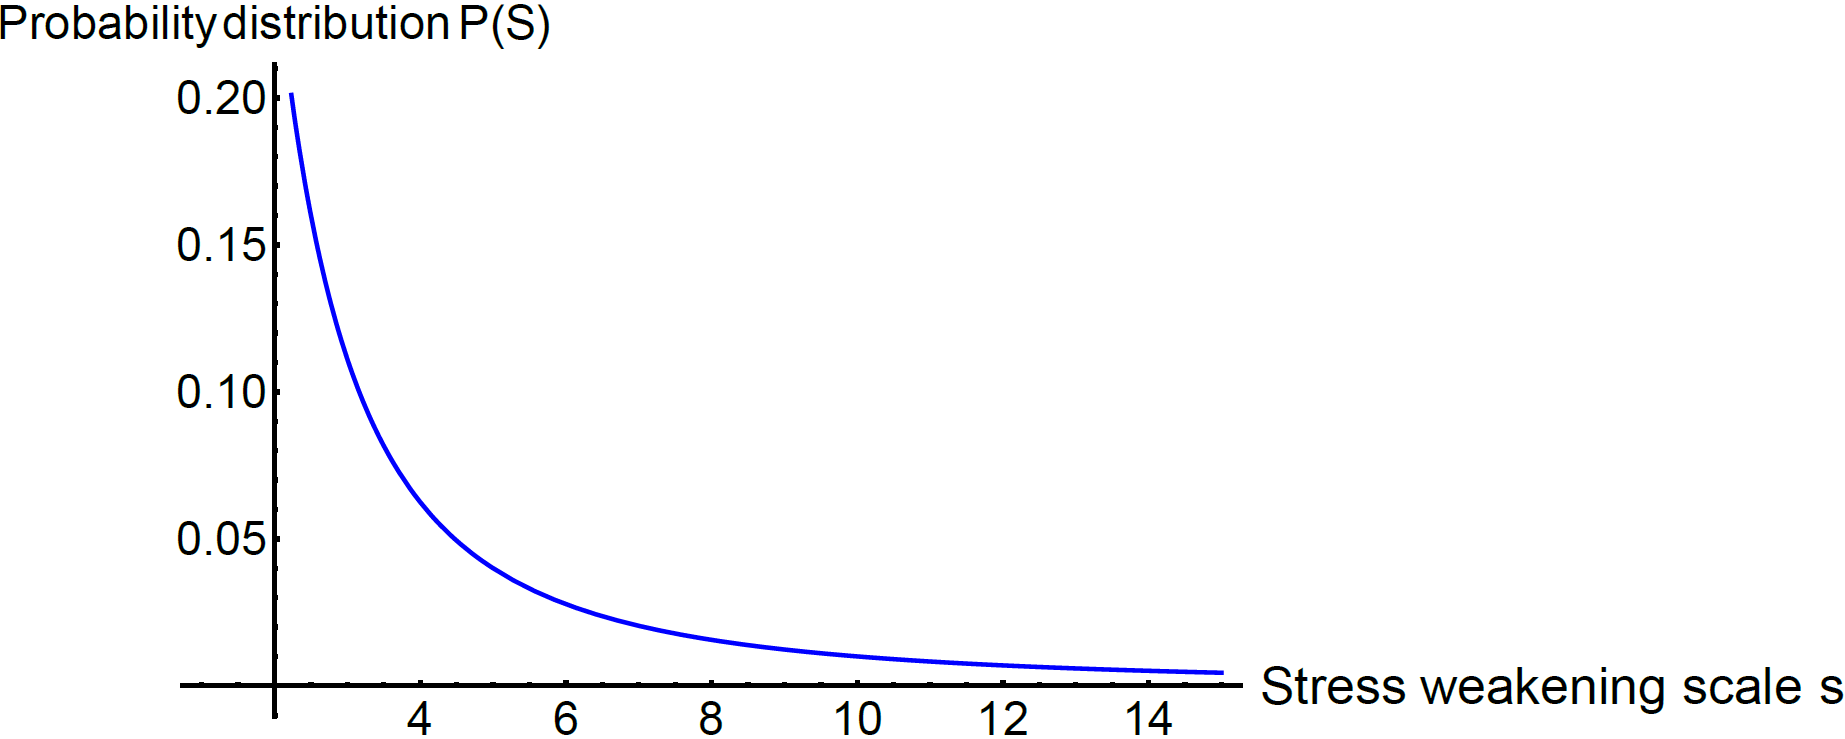
\includegraphics[width=\textwidth]{figures//ps.png} 
		\caption{Weakening scales $s$ probability distribution curve}
		\label{ps}
	\end{figure}
\end{frame}	

\subsection{Yield function with mean stress effect}

\begin{frame}
	\frametitle{Mean stress effect}	
The idea is to consider Maitournam and Krebs' work that the yield limit $\sigma_y$ is reduced in presence of positive mean stress:
\begin{equation}
f\left(s\right)=||\uline{\uline{S}}(s)-\uline{\uline{b}}(s)||+\left( \lambda \Sigma_H-\sigma_y\right) /s\leqslant 0
\label{yieldfun}
\end{equation}
with $\uline{\uline{S}}(s)$ denoting the deviatoric part of the stress tensor at microscale, and $\uline{\uline{b}}(s)$ the corresponding backstress at the same scale.
\end{frame}	

\subsection{Local plastic model}
\begin{frame}
	\frametitle{Description of the mesoscopic stress state}	

\begin{itemize}
	\item $\dot{\uline{\uline{S}}}(s,M,t)=dev\dot{\uline{\uline{\Sigma}}}(M,t)-\dfrac{E}{1+\nu}\dot{\uline{\uline{\varepsilon}}}^p(s,M,t),$ Taylor-Lin scale transition model.

	\vspace{6pt}	
	\item
	$\dot{\uline{\uline{b}}}(s,M,t)=\dfrac{kE}{E-k} \dot{\uline{\uline{\varepsilon}}}^p(s,M,t),$  kinematic hardening model.

	\vspace{6pt}	
		\item
		$\dot{\uline{\uline{\varepsilon}}}^p(s,M,t)=\gamma\dfrac{\partial f(s,M,t)}{\partial \uline{\uline{S}}}, $ associated plastic flow rule.
\end{itemize}

	\vspace{6pt}
The local dissipated energy rate per volume at weakening scales $s$  is given by:
$$\dot{w}(s,M,t)=(\uline{\uline{S}}-\uline{\uline{b}})(s,M,t):\uline{\uline{\dot{\varepsilon}}}^p(s,M,t).$$ 
\end{frame}

\section{Damage accumulation for cyclic loads}
\begin{frame}
	\frametitle{Uniaxial cyclic load}	
	\begin{figure}[h!]
		\centering
		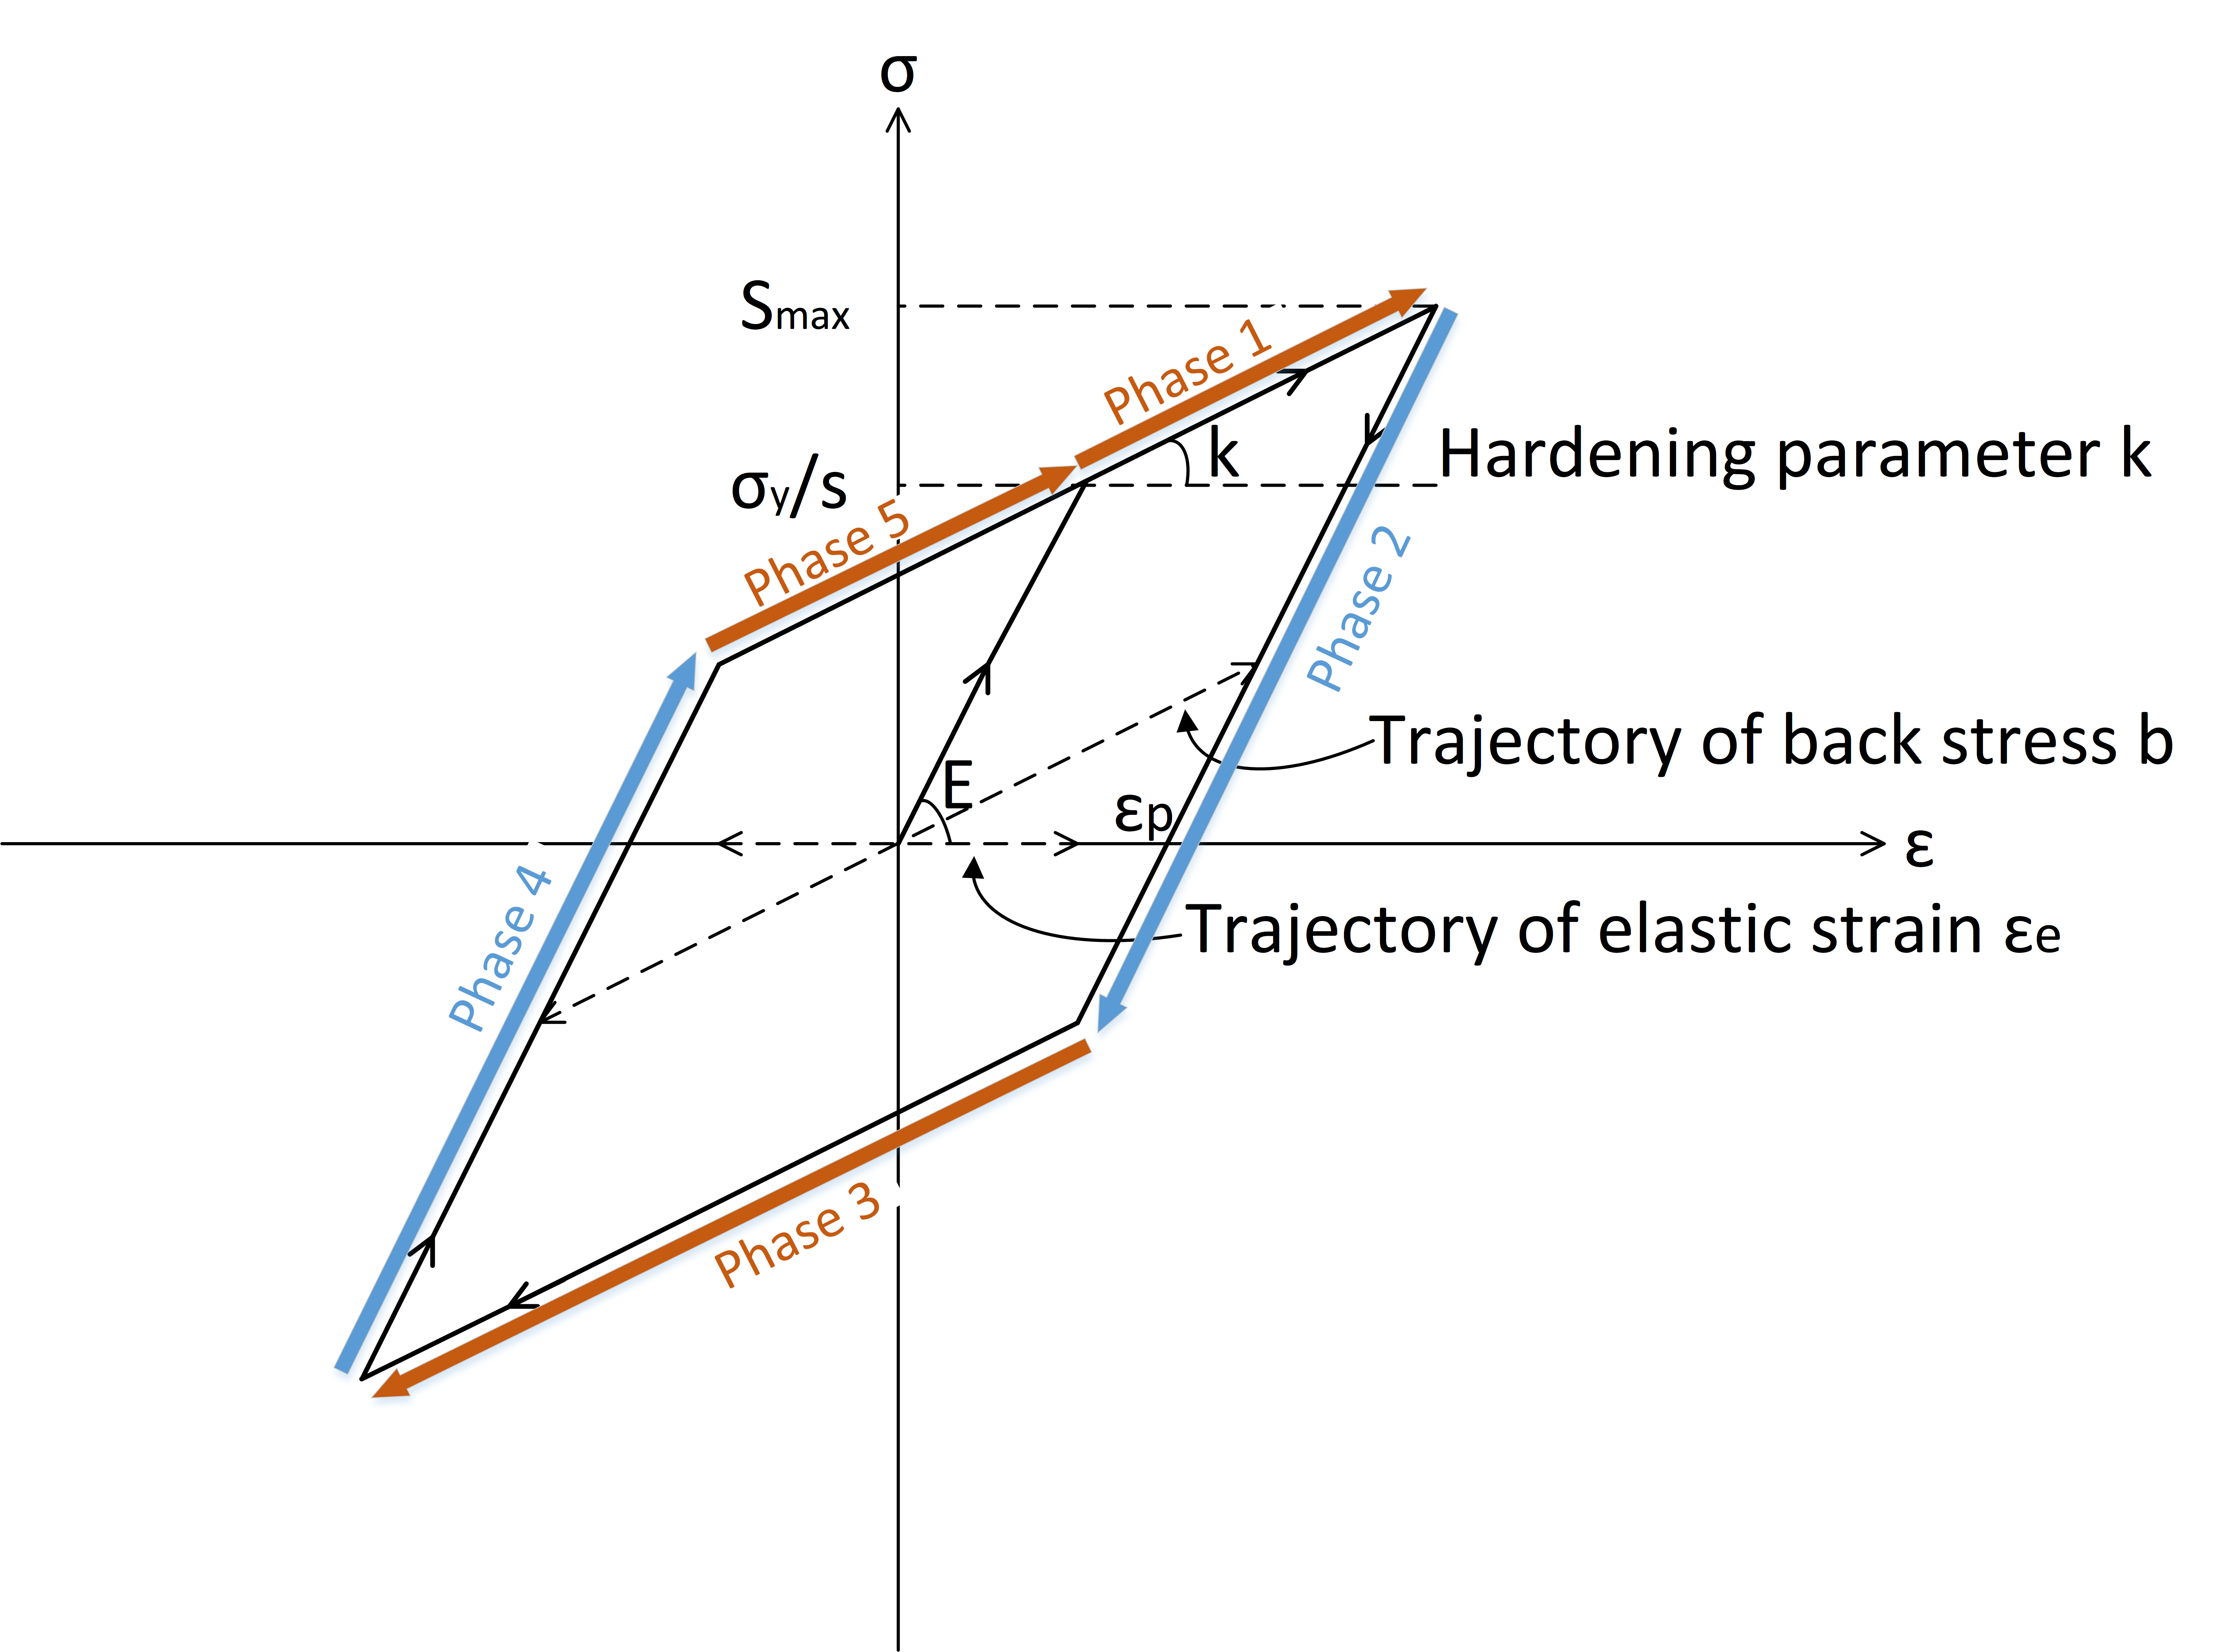
\includegraphics[width=0.9\textwidth]{figures//backstress.png} 
		\label{backstress}
	\end{figure}
\end{frame}	

\begin{comment}
\begin{frame}
	\frametitle{Description of the mesoscopic stress state}	
In uniaxial cyclic loading, there will be 3 kinds of loading patterns:
\begin{enumerate}
	
	\item	Elastic regime, in phase 2 and 4,where $\dot{\uline{\uline{\varepsilon}}}^p(s,M,t)=0$ ,  and $|\uline{\uline{S}}-\uline{\uline{b}}|<\left( \sigma_y-\lambda \Sigma_H\right)/s. $ 
	\vspace{6pt}
	
	\item Plastic regime according to plastic flow rule, with increasing plastic deformation, in phase 5 and 1, where	$\dot{\uline{\uline{\varepsilon}}}^p(s,M,t)=\gamma\dfrac{\uline{\uline{S}}(s)-\uline{\uline{b}}(s)}{||\uline{\uline{S}}(s)-\uline{\uline{b}}(s)||}> 0$ with  $\gamma=\left( dev\dot{\Sigma}\right)\left(\dfrac{kE}{E-k}+\dfrac{E}{1+\nu} \right) ^{-1}$ ,  with $\uline{\uline{S}}-\uline{\uline{b}}=\left( \sigma_y-\lambda \Sigma_H\right)/s$ and $\dot{\uline{\uline{S}}}-\dot{\uline{\uline{b}}}=0.$ 
	\vspace{6pt}
	
	\item Plastic regime in the other direction, in phase 3, there is	$\dot{\uline{\uline{\varepsilon}}}^p(s,M,t)<0$,  then $\uline{\uline{S}}-\uline{\uline{b}}=-\left( \sigma_y-\lambda \Sigma_H\right)/s$ and $\dot{\uline{\uline{S}}}-\dot{\uline{\uline{b}}}=0$ 
	
\end{enumerate}	

\end{frame}	
\end{comment}



\begin{frame}
	\frametitle{Cyclic load calculation}	
	\begin{block}{Energy dissipation at one scale s}
		\begin{itemize}
			\item $dW=(S-b)d\varepsilon^p=\dfrac{(E-k)(1+\nu) }{E(E+k\nu)}\dfrac{\sigma_y-\lambda \Sigma_H}{s}\left(S_{max}-\dfrac{\sigma_y-\lambda \Sigma_H}{s}\right)
			$ (phase 1)
			
			\vspace{6pt}
			\item $dW(phase 1)=dW(phase 5)=\dfrac{1}{2}dW(phase 3).$
	    \end{itemize}	
	\end{block}
\end{frame}	

	\begin{frame}
		\frametitle{Cyclic load calculation}	
	\begin{block}{Total dissipated energy $W$  at all scales during one cycle}
		\begin{equation}
		\begin{split}
		W_{cyc}&=4\int_{\left( \sigma_y-\lambda \Sigma_H\right) /S_{max}}^{\infty}dW(s,M,t)P(s)ds
		\\&=\dfrac{4(E-k)(1+\nu)\left( \beta-1\right) }{ E(E+k\nu)\beta\left( \beta+1\right) }\dfrac{S_{max}^{\beta+1}}{\left( \sigma_y-\lambda \Sigma_H\right) ^{\beta-1}}.
		\end{split}
		\end{equation}
	\end{block}
	\begin{block}{Damage law}
		\begin{equation}
D=f\left(\dfrac{W_{cyc}}{W_F} \right) 
		\end{equation}
	\end{block}
\end{frame}	


\section{Damage accumulation in general case}
\begin{frame}
	\frametitle{Generalized damage accumulation}	
	We combine a damage incremental law with increment of dissipated energy per unit time:
	\begin{block}{Damage incremental law}	
\begin{equation}
	\delta [1-(1-D)^{\gamma+1}]^{1-\alpha}=\dfrac{\dot{W}}{W_F}\delta t.
	\label{dt}
\end{equation}
	\end{block}
	$W_F$ is the energy threshold of the material.	
		\begin{block}{Multi-scale dissipated energy}	
\begin{equation}\dot{W}(M,t)=\int_{s=1}^{\infty}\dot{w}(s,M,t)P(s)ds=\int_{s=1}^{\infty}\left(\uline{\uline{S}}-\uline{\uline{b}} \right) (s,M,t):\uline{\uline{\dot{\varepsilon}^p}}(s,M,t)P(s)ds.
\end{equation}
		\end{block}
		Failure when D=1.
\end{frame}	

\section{Loop on time and scales}
\subsection{Integration rules for $\dot{W}$ and $\delta D$}

\begin{frame}
\frametitle{Integration rules}
	\begin{block}{}	
\begin{itemize}
\item No cycle counting. Only dissipated energy integration.
					
\vspace{6pt}
\item Gaussian quadrature rule for scale integration, time implicit for dissipated energy.

\end{itemize}	
\end{block}
\end{frame}	

\subsection{Regime determination under multiple scales}
\begin{frame}
	\frametitle{Regime determination}
	The material could be both in elastic and plastic regime at different scales.
	\begin{block}{Elastic regime:}	
\noindent
There we have
$\dot{\uline{\uline{\varepsilon}}}^p=0$, $\dot{\uline{\uline{b}}}=0$ and $\dot{\uline{\uline{S}}}=dev\dot{\uline{\uline{\Sigma}}}$, so
$$\dot{\uline{\uline{S}}}-\dot{\uline{\uline{b}}}=dev\dot{\uline{\uline{\Sigma}}},$$ 
yielding
\begin{equation}
\left( \uline{\uline{S}}-\uline{\uline{b}}\right) (t+dt)=\left( \uline{\uline{S}}-\uline{\uline{b}}\right) (t)+dev\dot{\uline{\uline{\Sigma}}}dt:=\left(  \uline{\uline{S}}-\uline{\uline{b}}\right)_{trial}(t+dt).
\label{trial}
\end{equation}
We are in elastic regime at scale $s$ as long as we satisfy
$$\left( \uline{\uline{S}}-\uline{\uline{b}}\right) (t+dt)\leqslant\left( \sigma_y-\lambda \Sigma_H\right)/s.$$	
	\end{block}
\end{frame}	


\begin{frame}
	\frametitle{Regime determination and damage integration}
	\begin{block}{Final expression of energy dissipation during time step dt }	
	\begin{equation}
	\begin{split}
	W&=\dot{W}dt
	\\&=\frac{1}{2}\sum_{i}\omega_i\dot{w}\left[  \left( \frac{x+1}{2}\right) ^{\frac{1}{1-\beta}}\right]dt
	\\&=\dfrac{(E-k)(1+\nu) }{2E(E+k\nu)}\sum_{i}\omega_i\left\langle  \left| \left|\uline{\uline{S}}-\uline{\uline{b}}\right| \right|_{trial}-\dfrac{\sigma_y-\lambda \Sigma_H}{\left( \dfrac{x_i+1}{2}\right) ^{\frac{1}{1-\beta}}}\right\rangle \dfrac{\sigma_y-\lambda \Sigma_H}{\left( \dfrac{x_i+1}{2}\right) ^{\frac{1}{1-\beta}}}.
	\end{split}
	\label{finaldw}
	\end{equation}
	\end{block}
We use 25 Gauss Legendre points in numerical integration.

$$g_{n+1}=g_n+\dfrac{\dot{W}dt}{W_F}=g_n+\dfrac{W}{W_F},$$

with $D_n=\left[1-\left(1-g_n^{\frac{1}{1-\alpha}} \right)^{\frac{1}{\gamma+1}}  \right] $.

\end{frame}	

\section{Application}
\subsection{One dimensional application to simple cyclic data}

\begin{frame}
	\frametitle{Material parameters}
	The test is performed on a sinusoidal axial load $\Sigma=Csin(t)$, giving the deviatoric amplitude $S_{max}=\sqrt{\dfrac{2}{3}}C$.
\begin{table}[!h]
	\centering
	\begin{tabular}{ll}
		\hline
		\textbf{Parameters}                                         & \textbf{Value}                    \\ \hline
		Load                                                              & $\Sigma=5e8sin(t)$ Pa                  \\
		Young's modulus                                             & $E=2e11$ Pa                       \\
		Hardening parameter                                         &  $k=6e8$ Pa \\
		Weakening scales distribution exponent                      & $\beta=3$                             \\
		Hydrostatic pressure sensitivity                            & $\lambda=0.5$                     \\
		Macroscopic yield stress                                    & $\sigma_y=6.38e8$ Pa              \\
		Mean stress                                        & $\Sigma_H=0$ Pa                     \\
		Material parameter from Chaboche law(Wohler curve exponent) & $\gamma=0.5$                        \\
		Non-linearity of damage accumulation & $\alpha=0.8$                        \\
		Initial damage                                              & $D=0$                          \\
		Initial time                                                & $t=0$ s                            \\
		Dissipated energy to failure per unit volume                & $W_F=3e6$ J                       \\
		Looping step                                           & 1e-4 s              \\ \hline
	\end{tabular}
	\caption{Material parameters in a simple cyclic load }
	\label{Sin}
\end{table}
\end{frame}	


\begin{frame}
	\frametitle{Sinusoidal test}
\begin{figure}[!h]
	\centering
	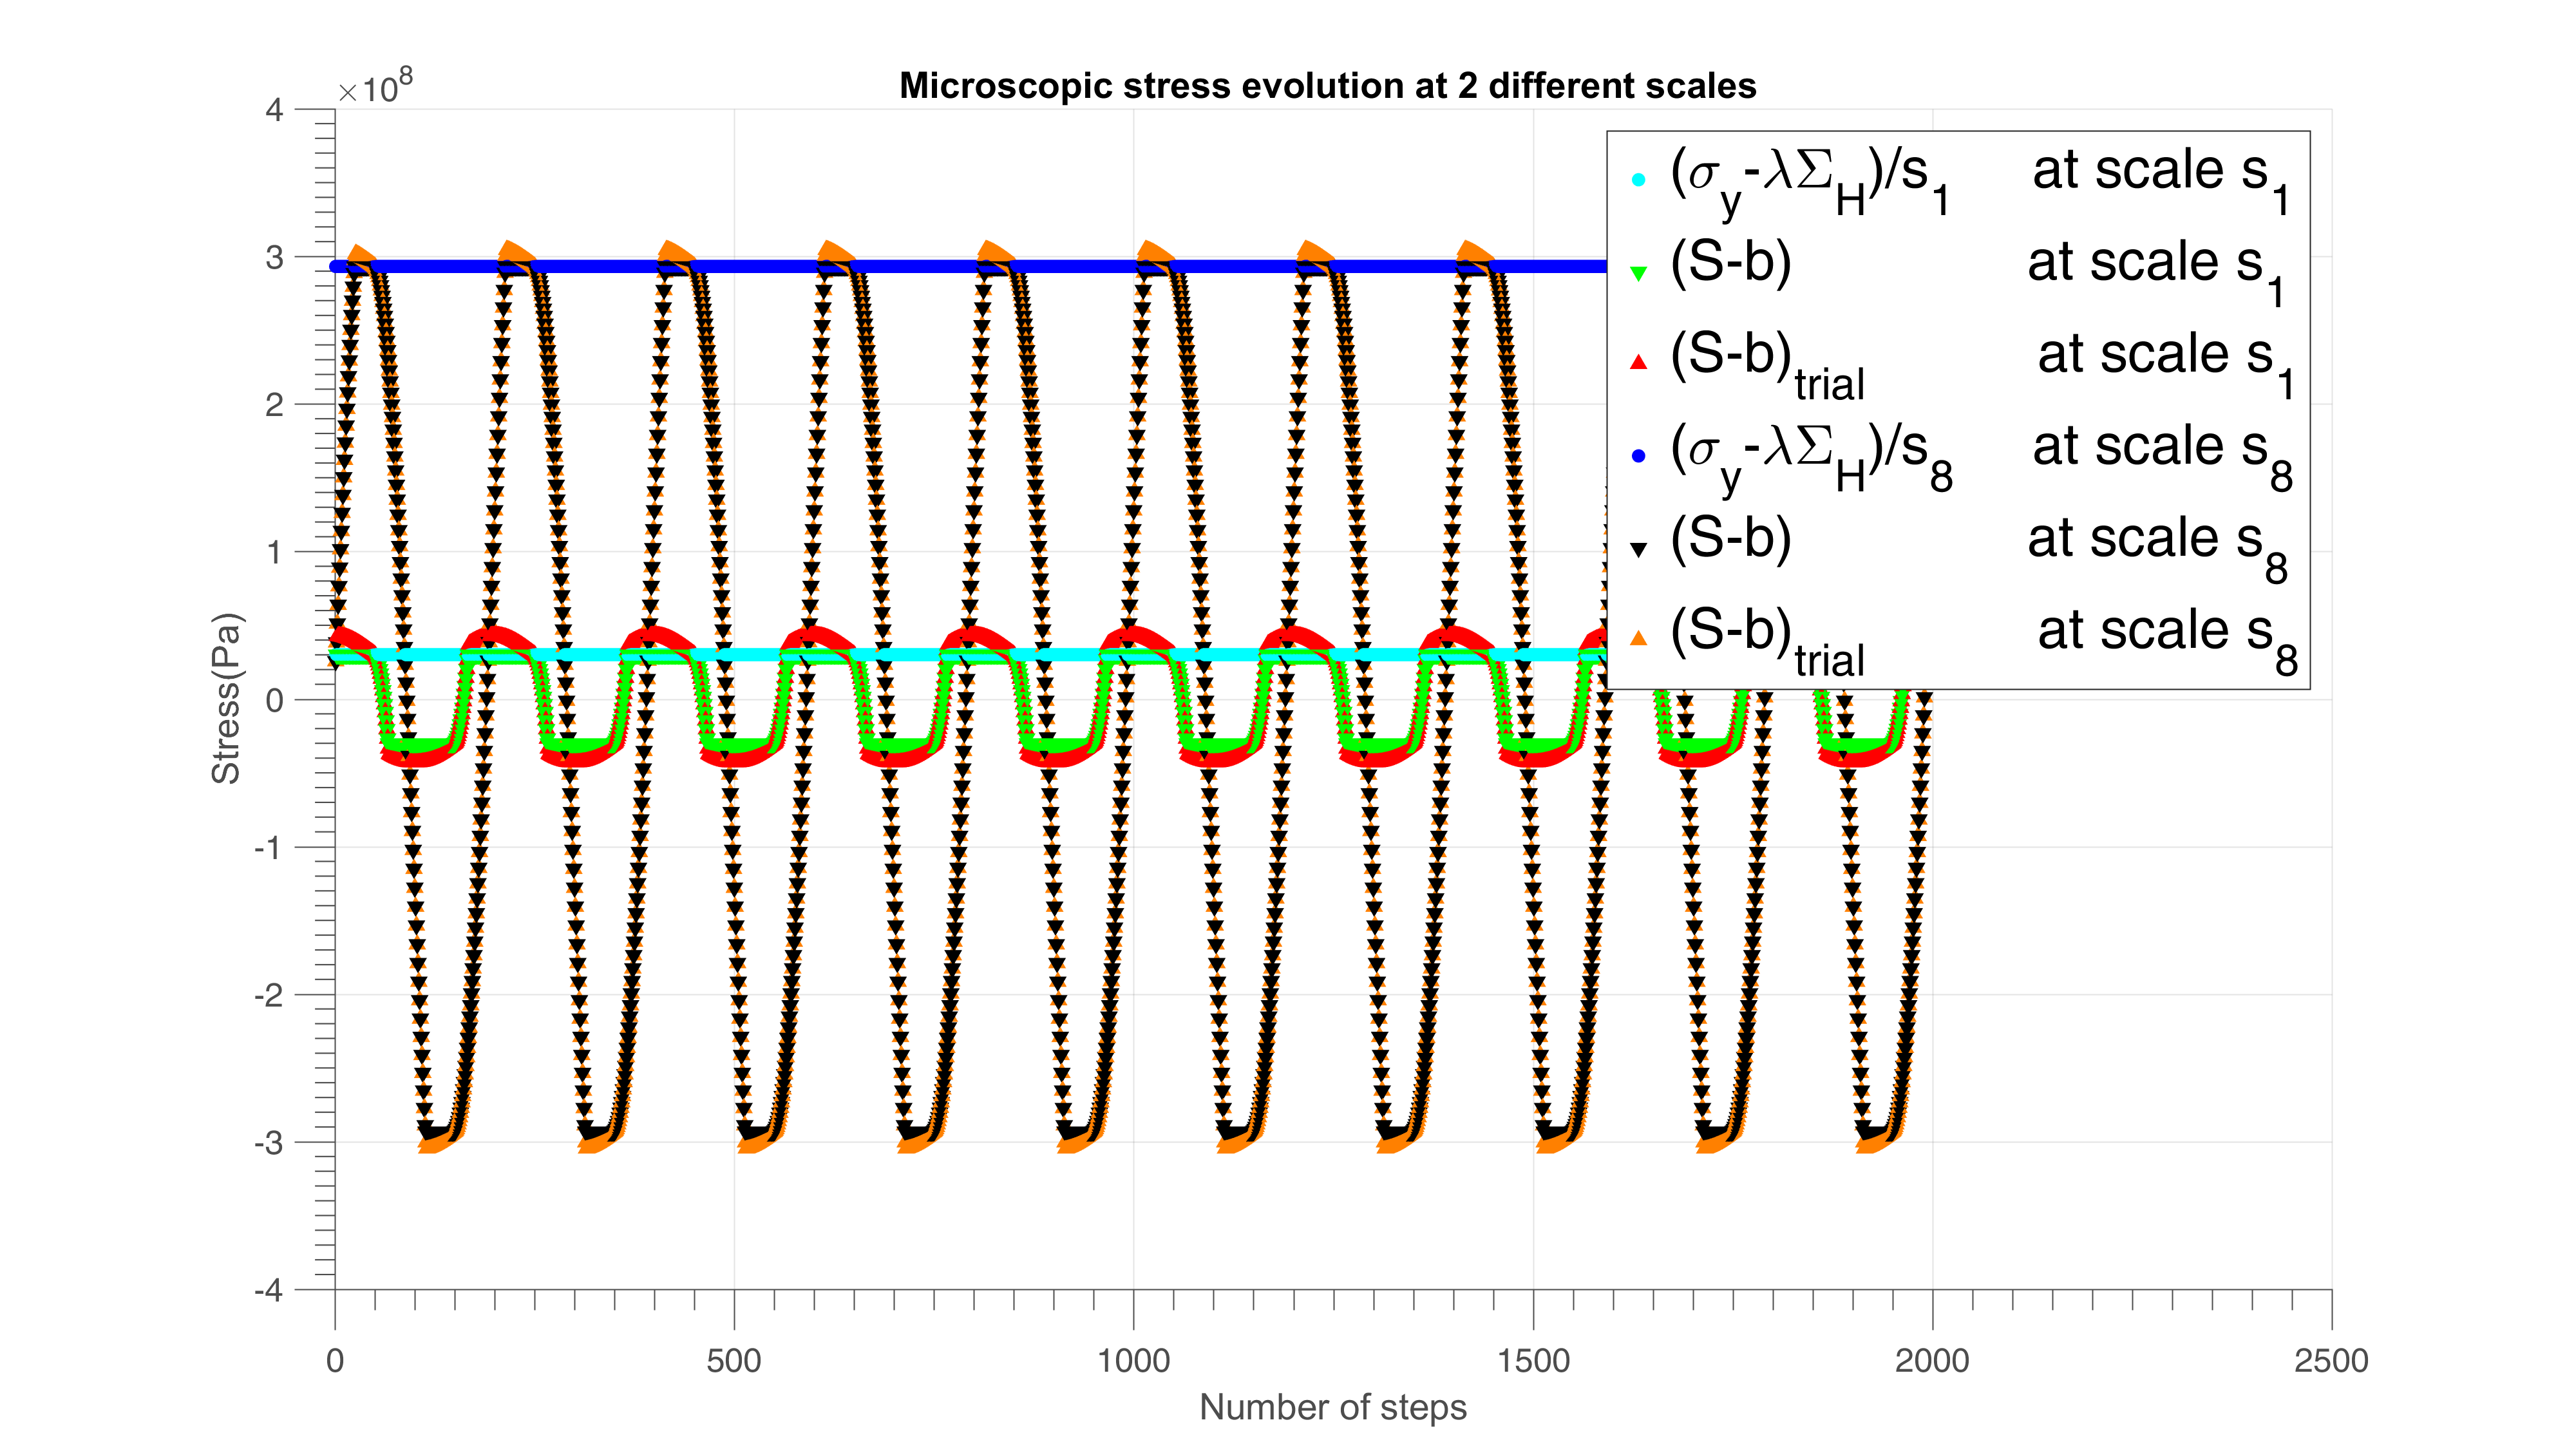
\includegraphics[width=\textwidth]{figures//trialsin.png} 
	\caption{Microscopic $\left( \uline{\uline{S}}-\uline{\uline{b}}\right)_{trial}$ and $\left( \uline{\uline{S}}-\uline{\uline{b}}\right)$ evolution with time under different weakening scales in sinusoidal load($s_1=21.21657929229650$ and $s_8=2.176132808422946$)}
	\label{trialsin}
\end{figure}
\end{frame}	
\begin{frame}
	\frametitle{Sinusoidal test}
\begin{figure}[!h]
	\centering
	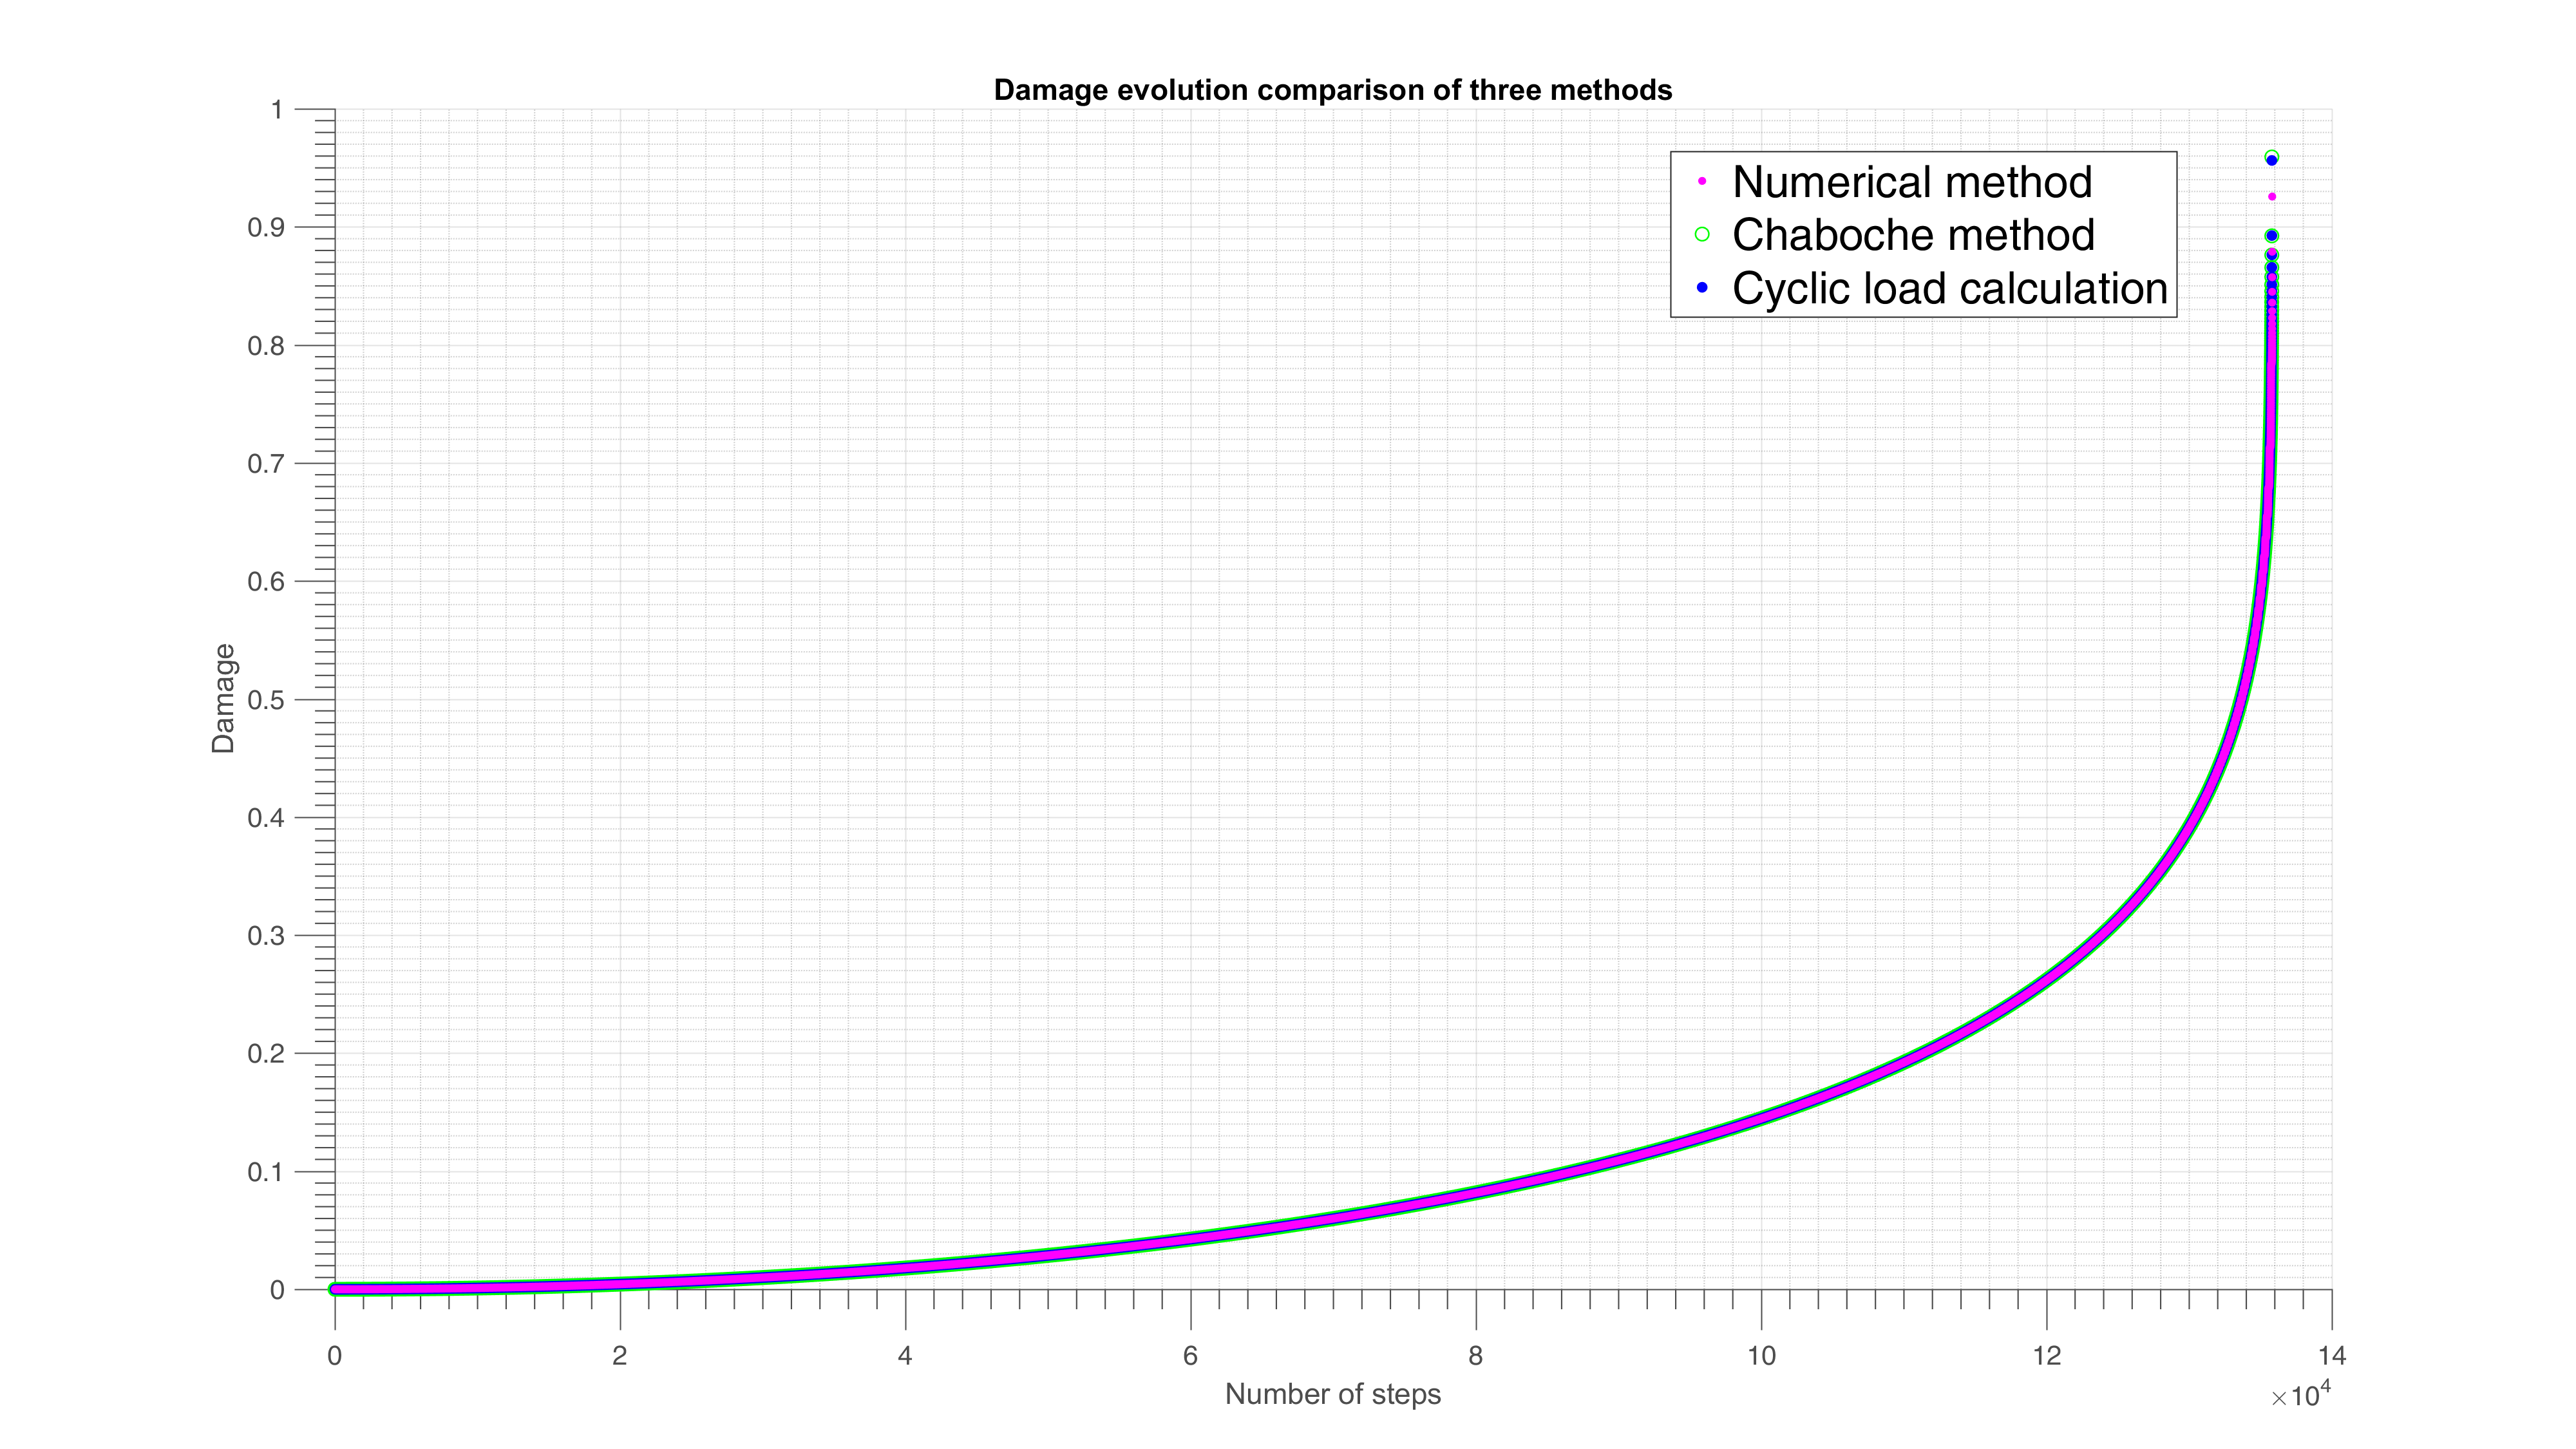
\includegraphics[width=\textwidth]{figures//damagesin.png} 
	\caption{Damage evolution with time under sinusoidal load with two different methods}
	\label{damsin}
\end{figure}
\end{frame}	

\subsection{One dimensional application to PSA data}

\begin{frame}
	\frametitle{One dimensional application}
\begin{figure}[!h]
	\centering
	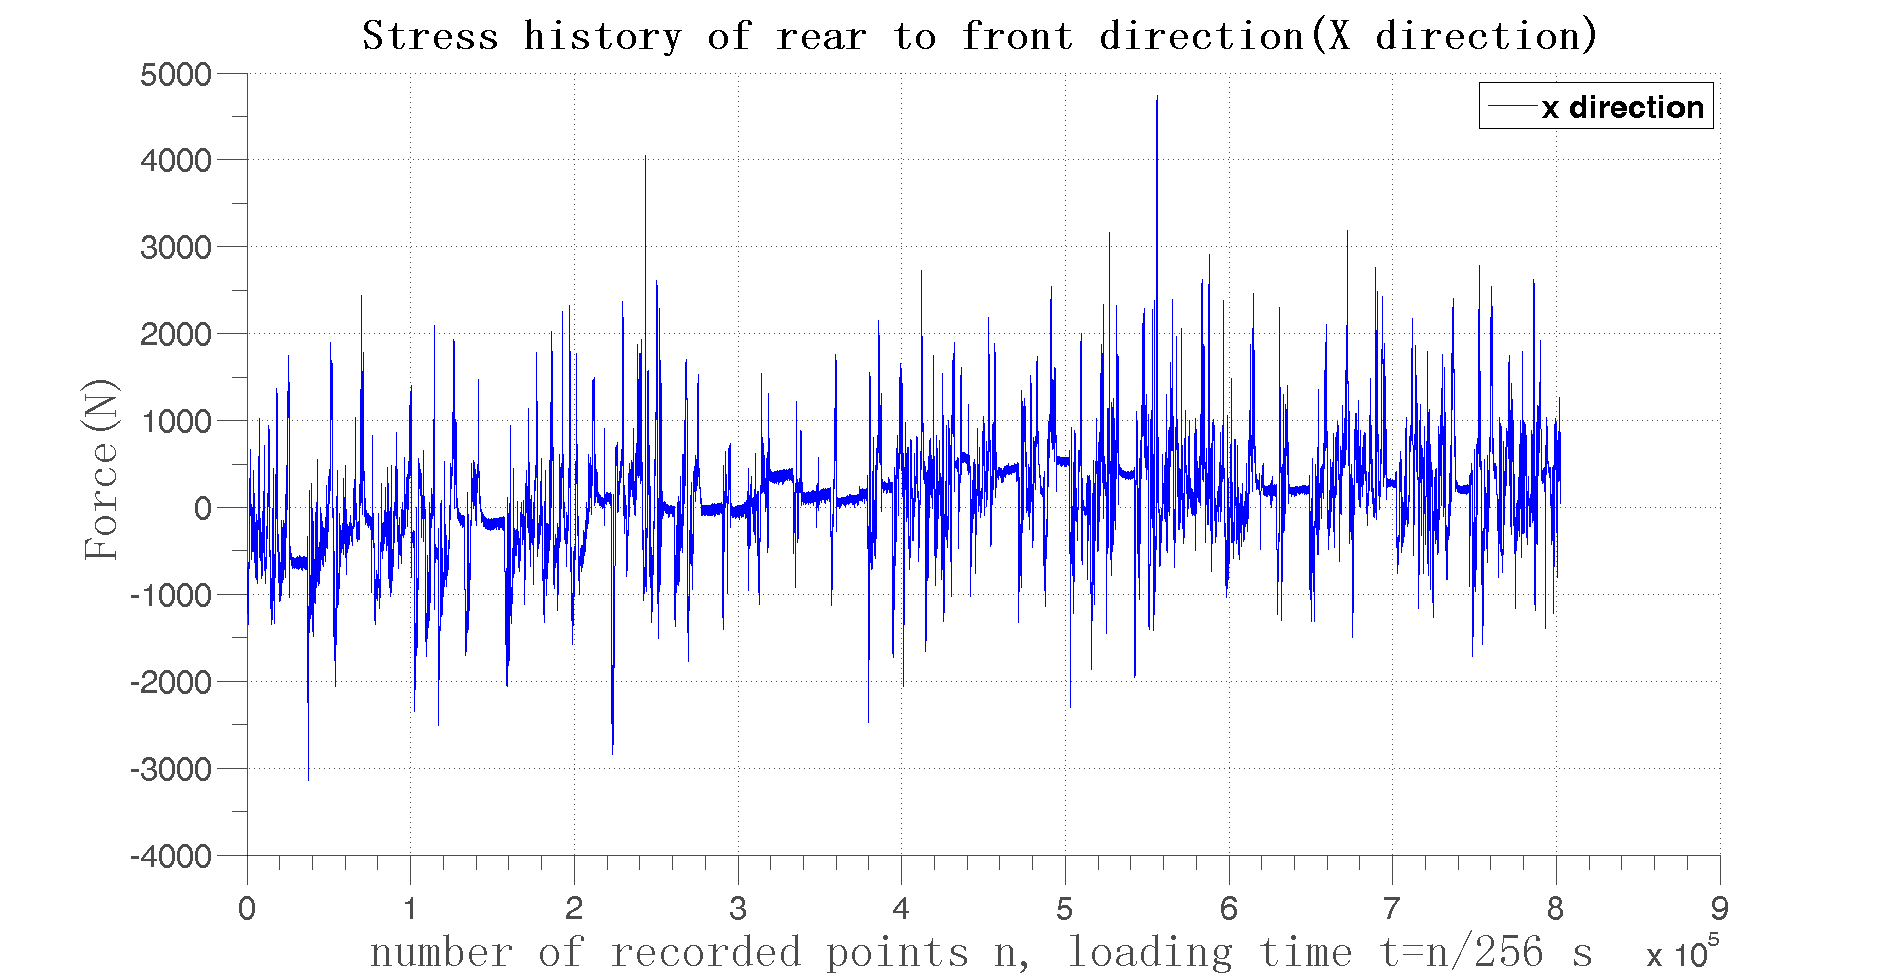
\includegraphics[width=\textwidth]{figures//x.png} 
	\caption{Loading history of X direction, force vs the record index n, with 256 sample recorded per second}
	\label{x}
\end{figure}
\end{frame}	


\begin{frame}
	\frametitle{One dimensional application}
\begin{figure}[!h]
	\centering
	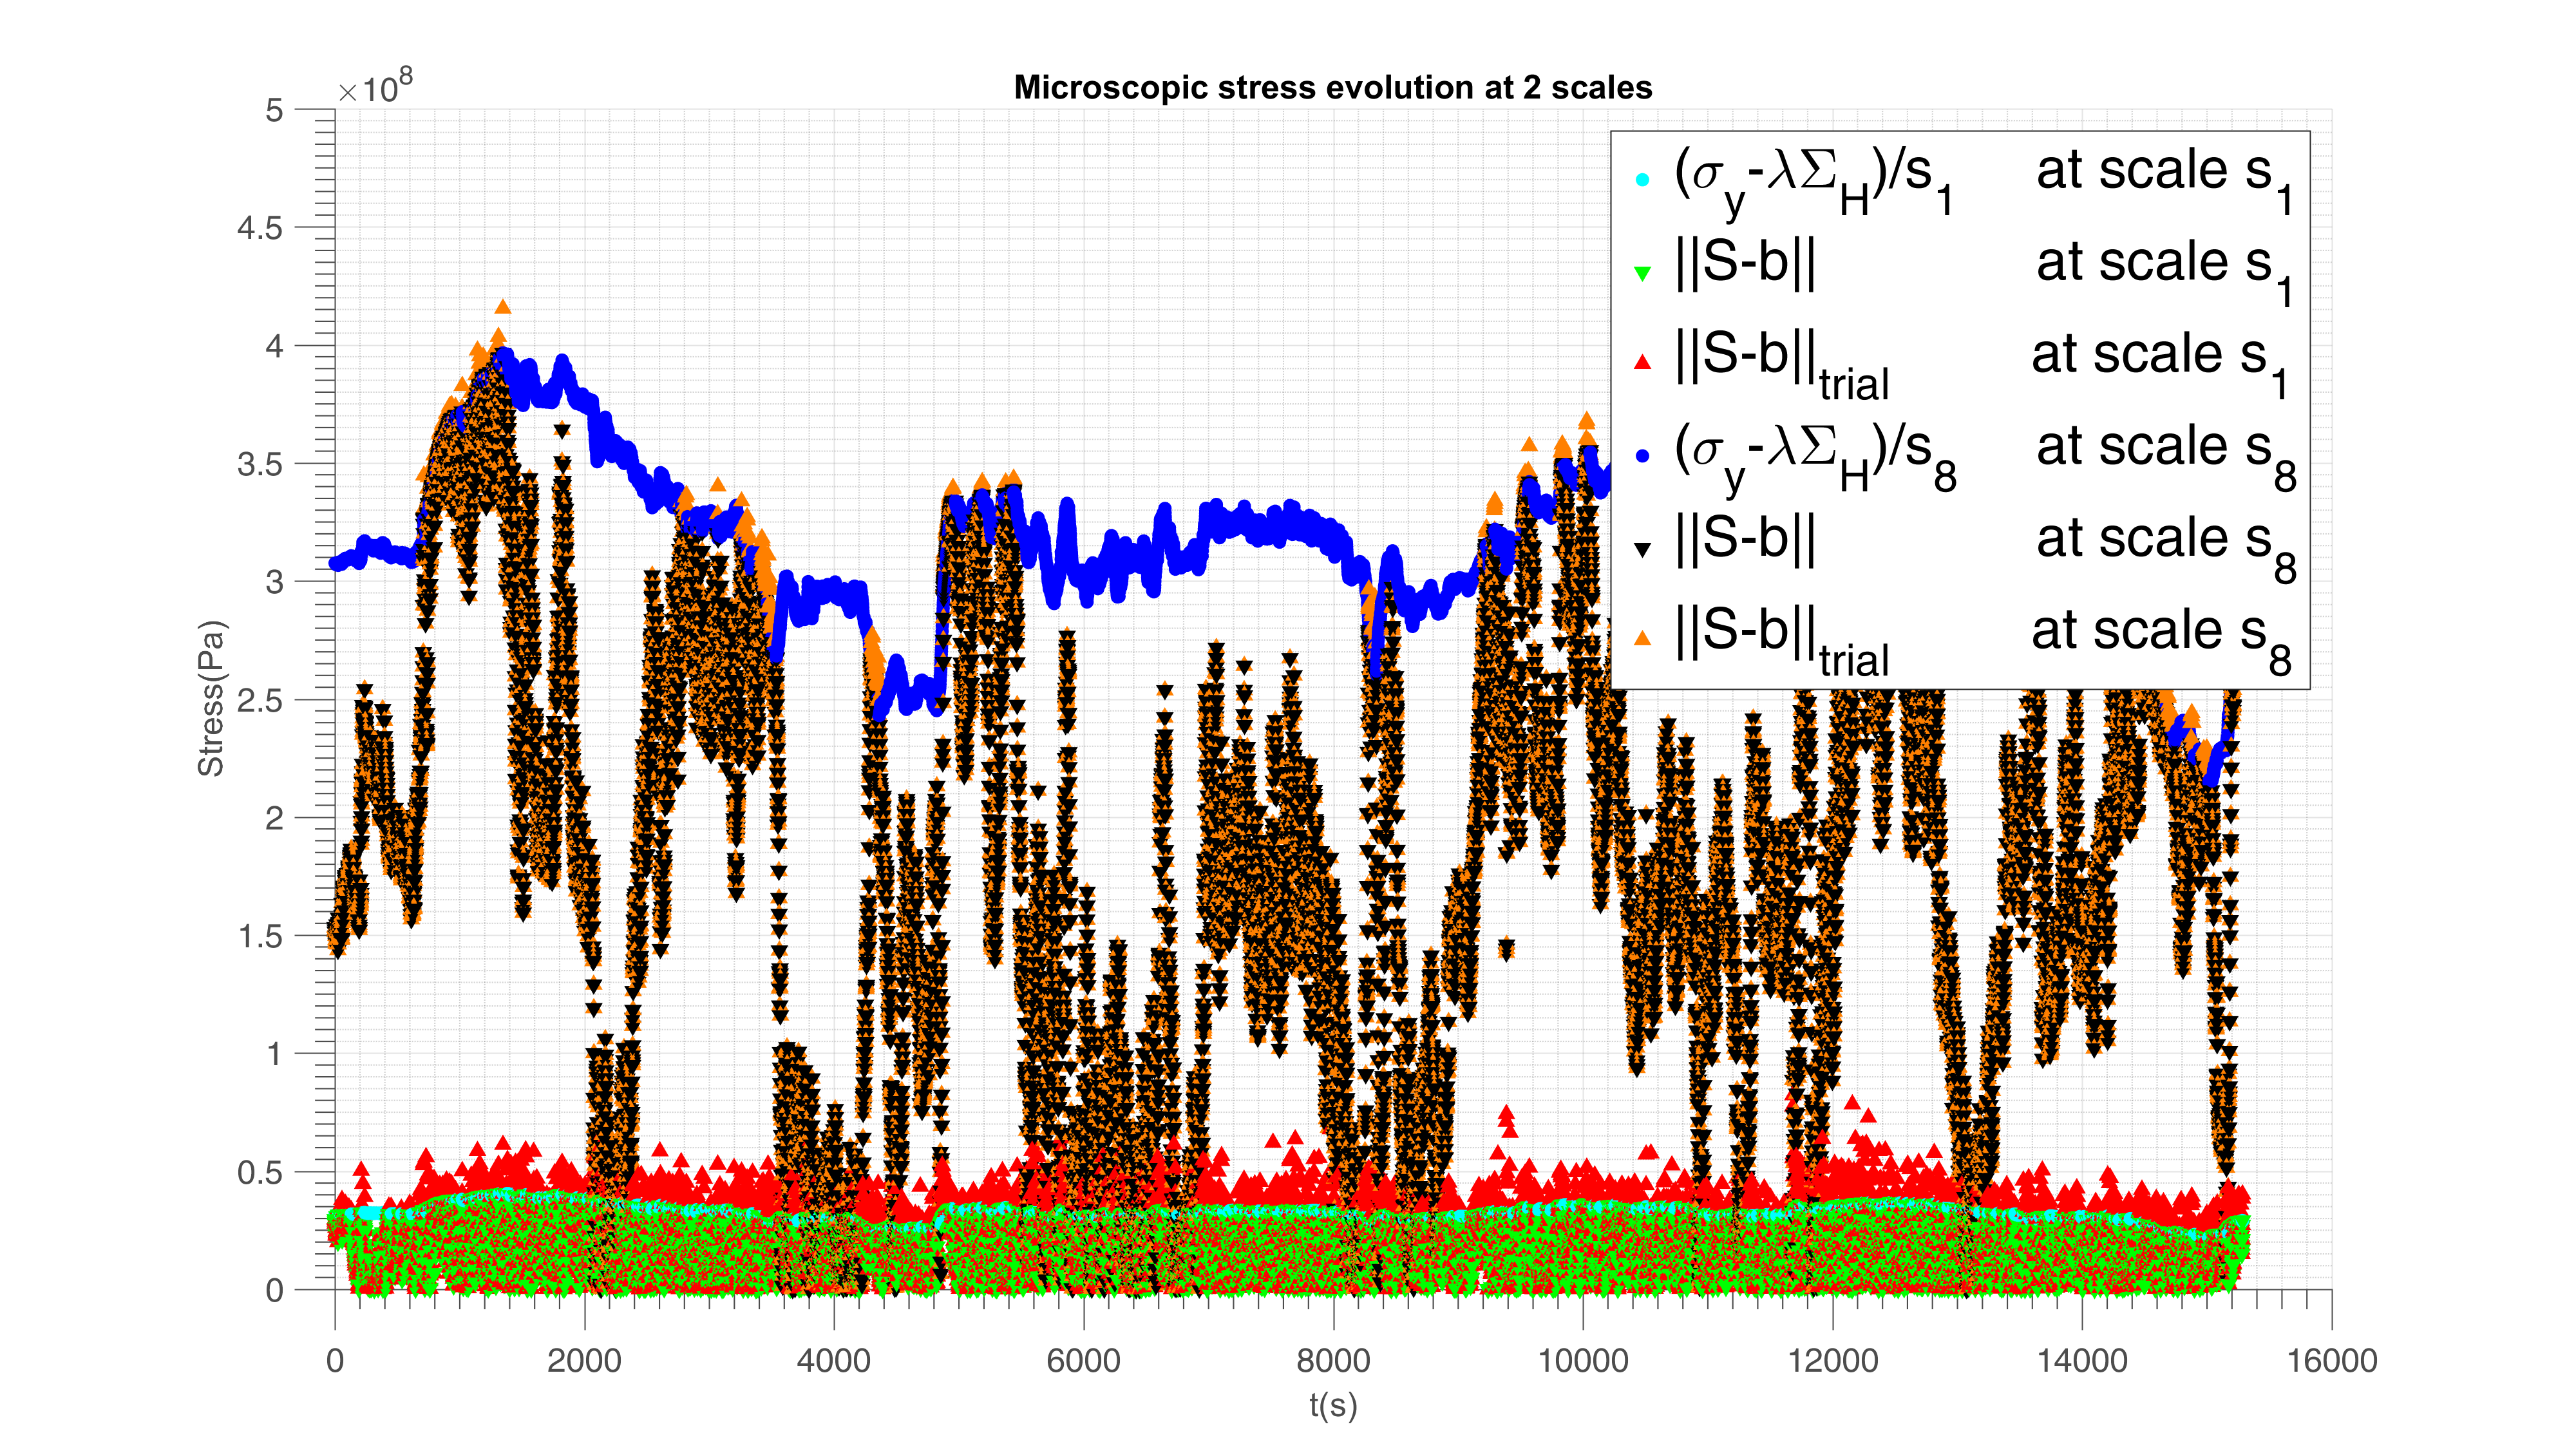
\includegraphics[width=\textwidth]{figures//trialreal1d1.png} 
	\caption{$\left\|  \uline{\uline{S}}-\uline{\uline{b}}\right\| _{trial}$ and $\left\| \uline{\uline{S}}-\uline{\uline{b}}\right\|$ evolution with time under different weakening scales in PSA load history}
	\label{trialreal}
\end{figure}
\end{frame}	

\begin{frame}
	\frametitle{One dimensional application}
	\begin{figure}[!h]
		\centering
		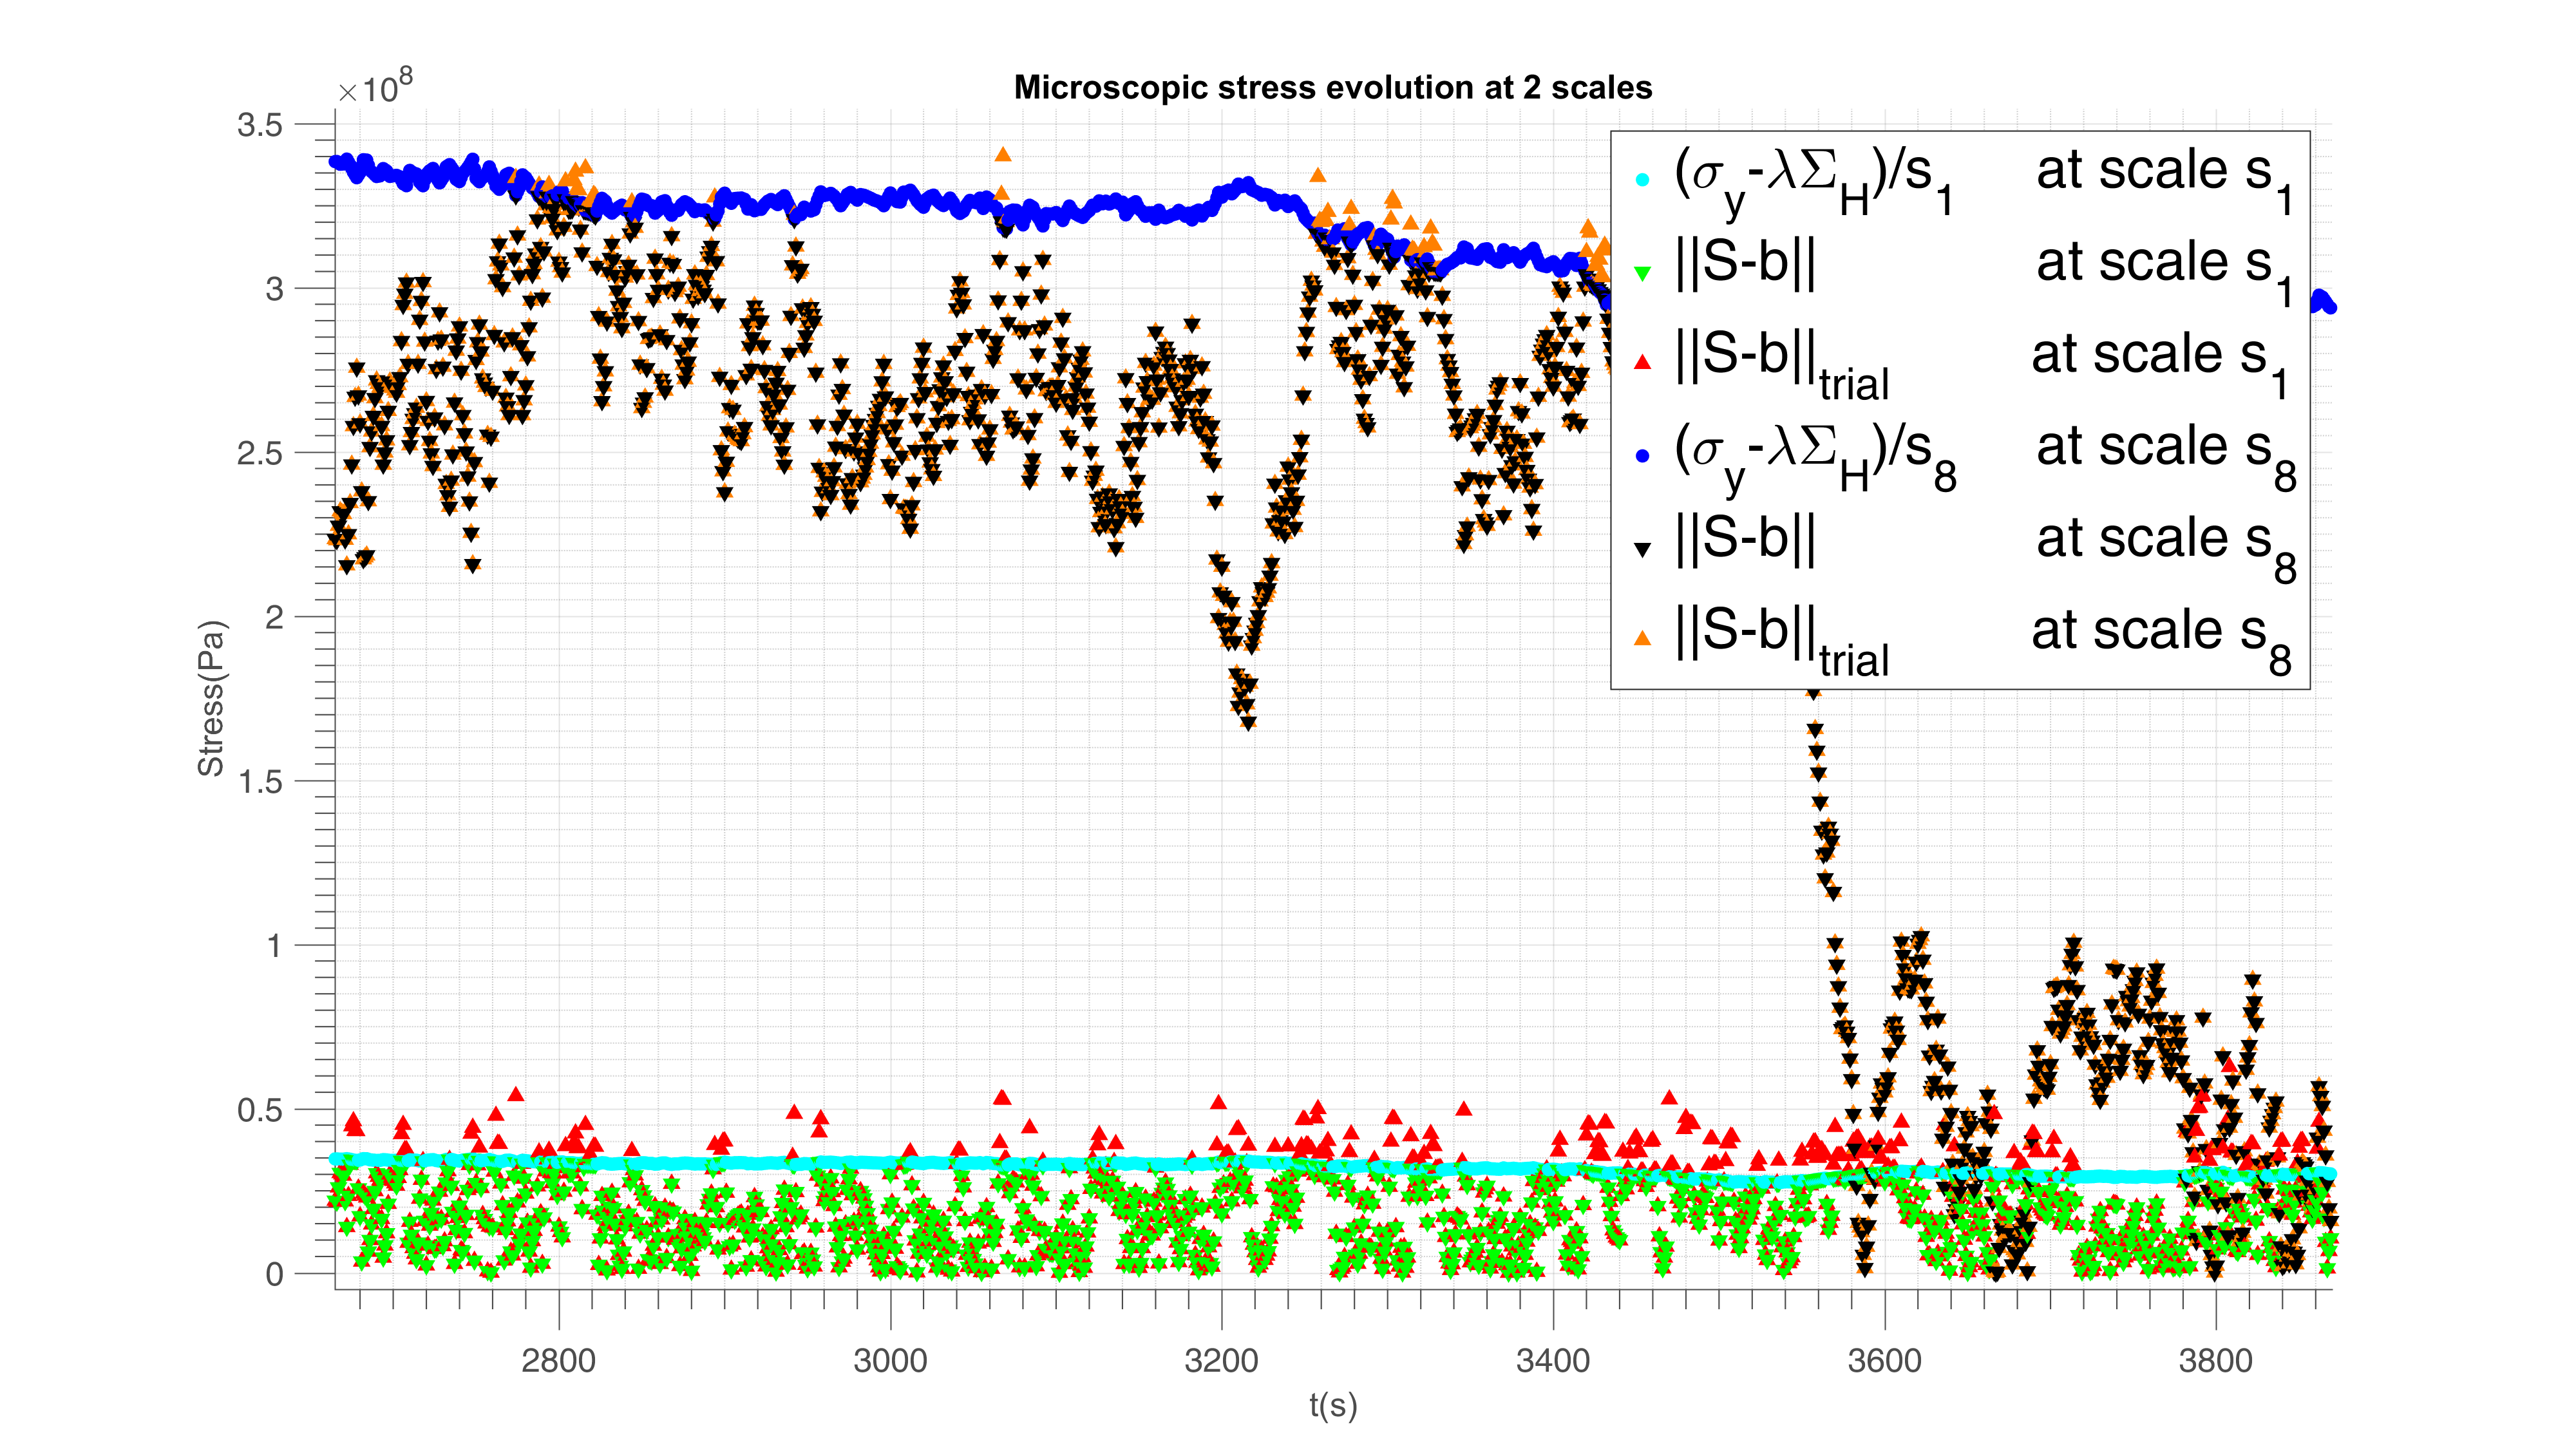
\includegraphics[width=\textwidth]{figures//trialreal1d2.png} 
		\caption{Circled area magnification where there is more $\left\| \uline{\uline{S}}-\uline{\uline{b}}\right\|_{trial}>\sigma_y$(plasticity) at scale $s_1$ than at $s_8$}
		\label{trialreal1d3}
	\end{figure}
\end{frame}	

\begin{frame}
	\frametitle{One dimensional application}
\begin{figure}[!h]
	\centering
	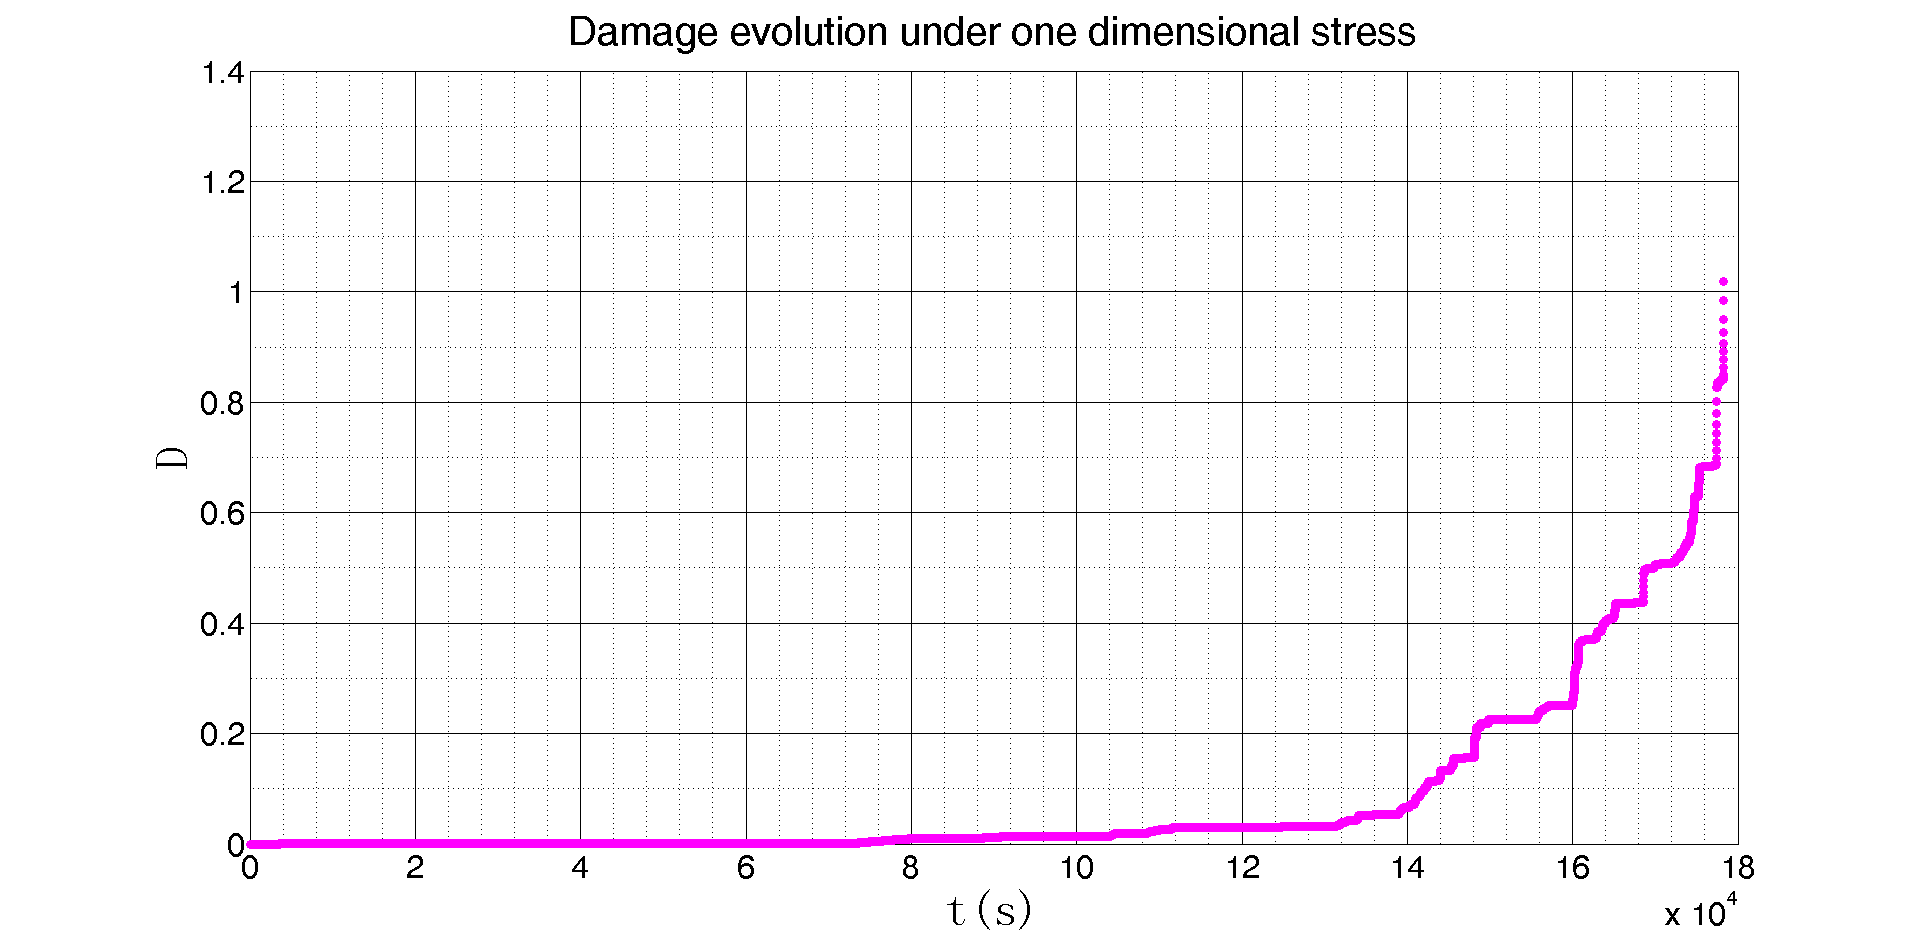
\includegraphics[width=\textwidth]{figures//damage1d.png} 
	\caption{Damage evolution with time at one dimension PSA load history}
	\label{damage1d}
\end{figure}
\end{frame}	



 \subsection{Multi-dimensional application to PSA data}
\begin{frame}
	\frametitle{Multi-dimensional application}
 \begin{figure}[!h]
 	\centering
 	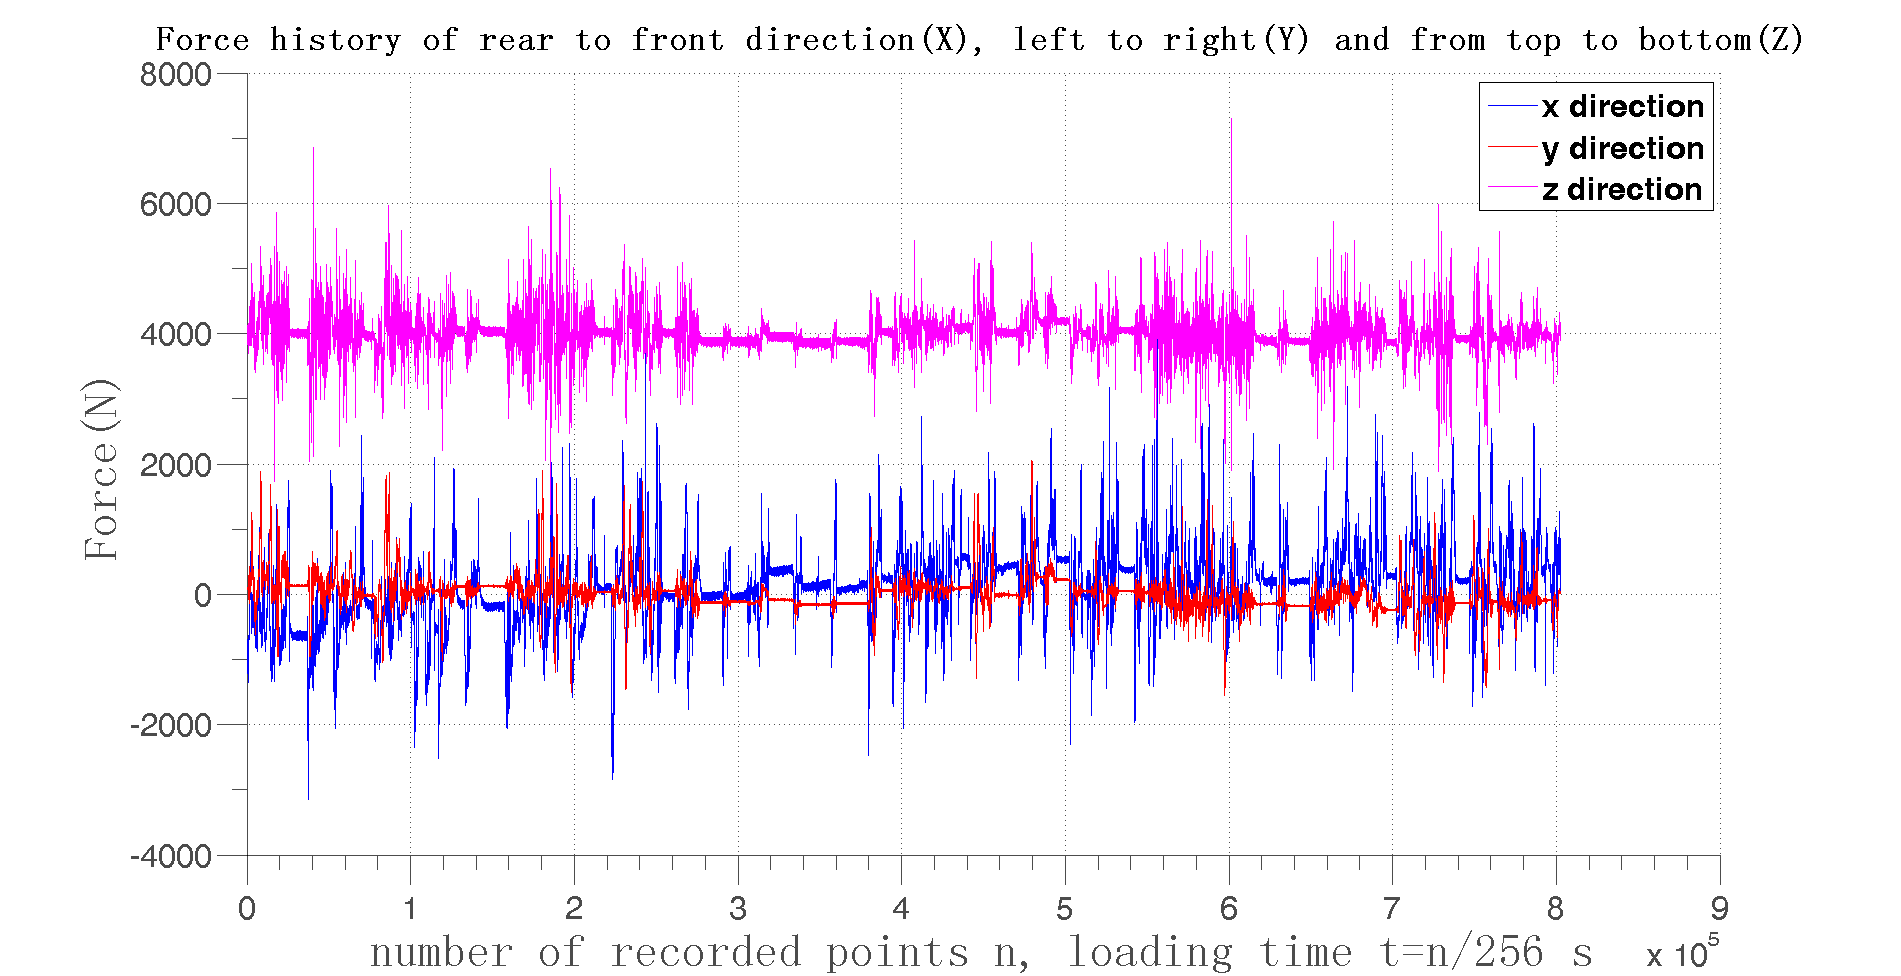
\includegraphics[width=\textwidth]{figures//xyz.png} 
 	\caption{Loading history of 3 different directions}
 	\label{xyz}
 \end{figure}
\end{frame}	

\begin{frame}
	\frametitle{Multi-dimensional application}
 In real case, the vertical force $F_z$ is much larger than the axial and horizontal forces $F_x$ and $F_y$. However, in order to investigate large domains of interest, we first scale the axial and horizontal forces to reach comparable impact and transform them in principal stresses $c_x\dfrac{F_x}{A}$ applied along the stress principle vector $\uline{e}_\alpha$(respectively $\uline{e}_\beta$) that we choose randomly. We therefore consider the following macroscopic stress tensor:
 \begin{equation}
 \uline{\uline{\Sigma}}=\dfrac{F_z(t)}{A}\uline{e}_1\otimes \uline{e}_1+c_x\dfrac{F_x(t)}{A}\uline{e}_{\alpha}\otimes \uline{e}_{\alpha}+c_y\dfrac{F_y(t)}{A}\uline{e}_{\beta}\otimes \uline{e}_{\beta}
 \label{tensor1}
 \end{equation}
 where $\uline{e}_{\alpha}$  and $\uline{e}_{\beta}$ are principal vectors whose spherical coordinate are $\theta_x$, $\varphi_x$,  $\theta_y$ and $\varphi_y$ respectively:
 $$\uline{e}_{\alpha}=cos\theta_x\uline{e}_1+sin\theta_xcos\varphi_x\uline{e}_2+sin\theta_xsin\varphi_x\uline{e}_3,$$
 $$\uline{e}_{\beta}=cos\theta_y\uline{e}_1+sin\theta_ycos\varphi_y\uline{e}_2+sin\theta_ysin\varphi_y\uline{e}_3.$$


\end{frame}

\begin{frame}
	\frametitle{Multi-dimensional application}
  \begin{figure}[!h]
  	\centering
  	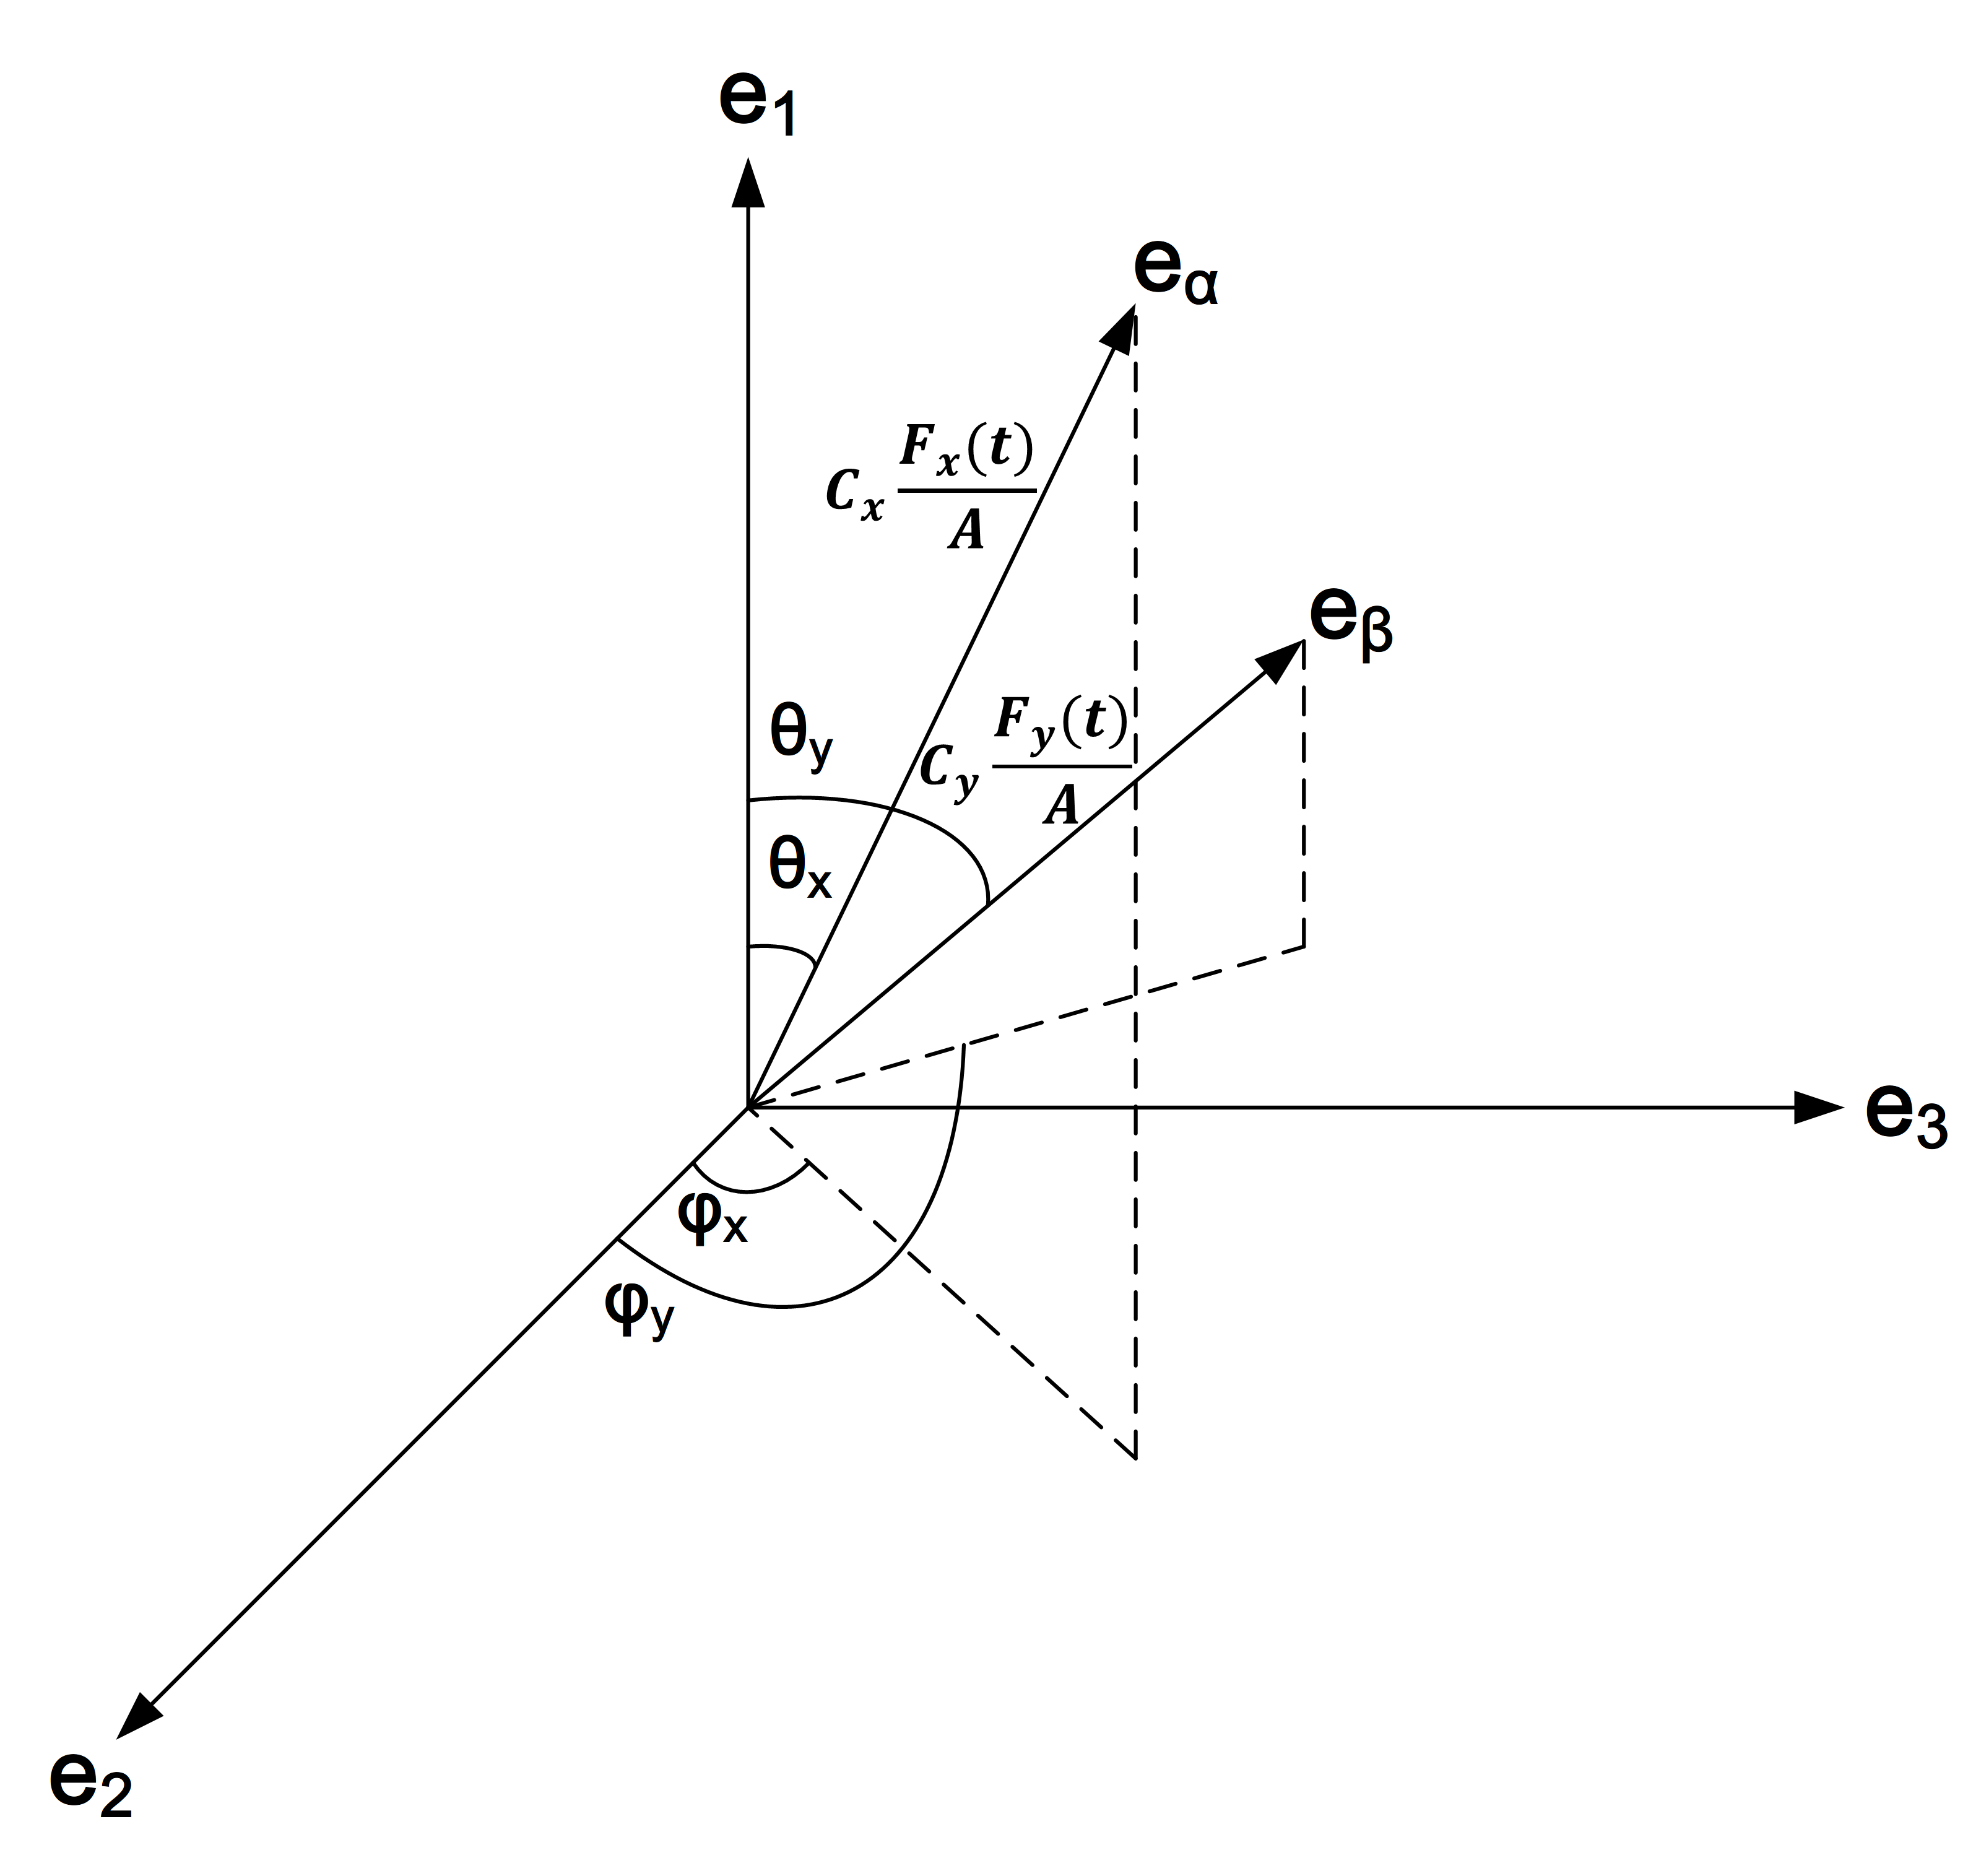
\includegraphics[width=0.7\textwidth]{figures//xab.png} 
  	\caption{Loading in 3 different directions}
  	\label{xab}
  \end{figure}
\end{frame}	

\begin{frame}
	\frametitle{Multi-dimensional application}
\begin{figure}[!h]
	\centering
	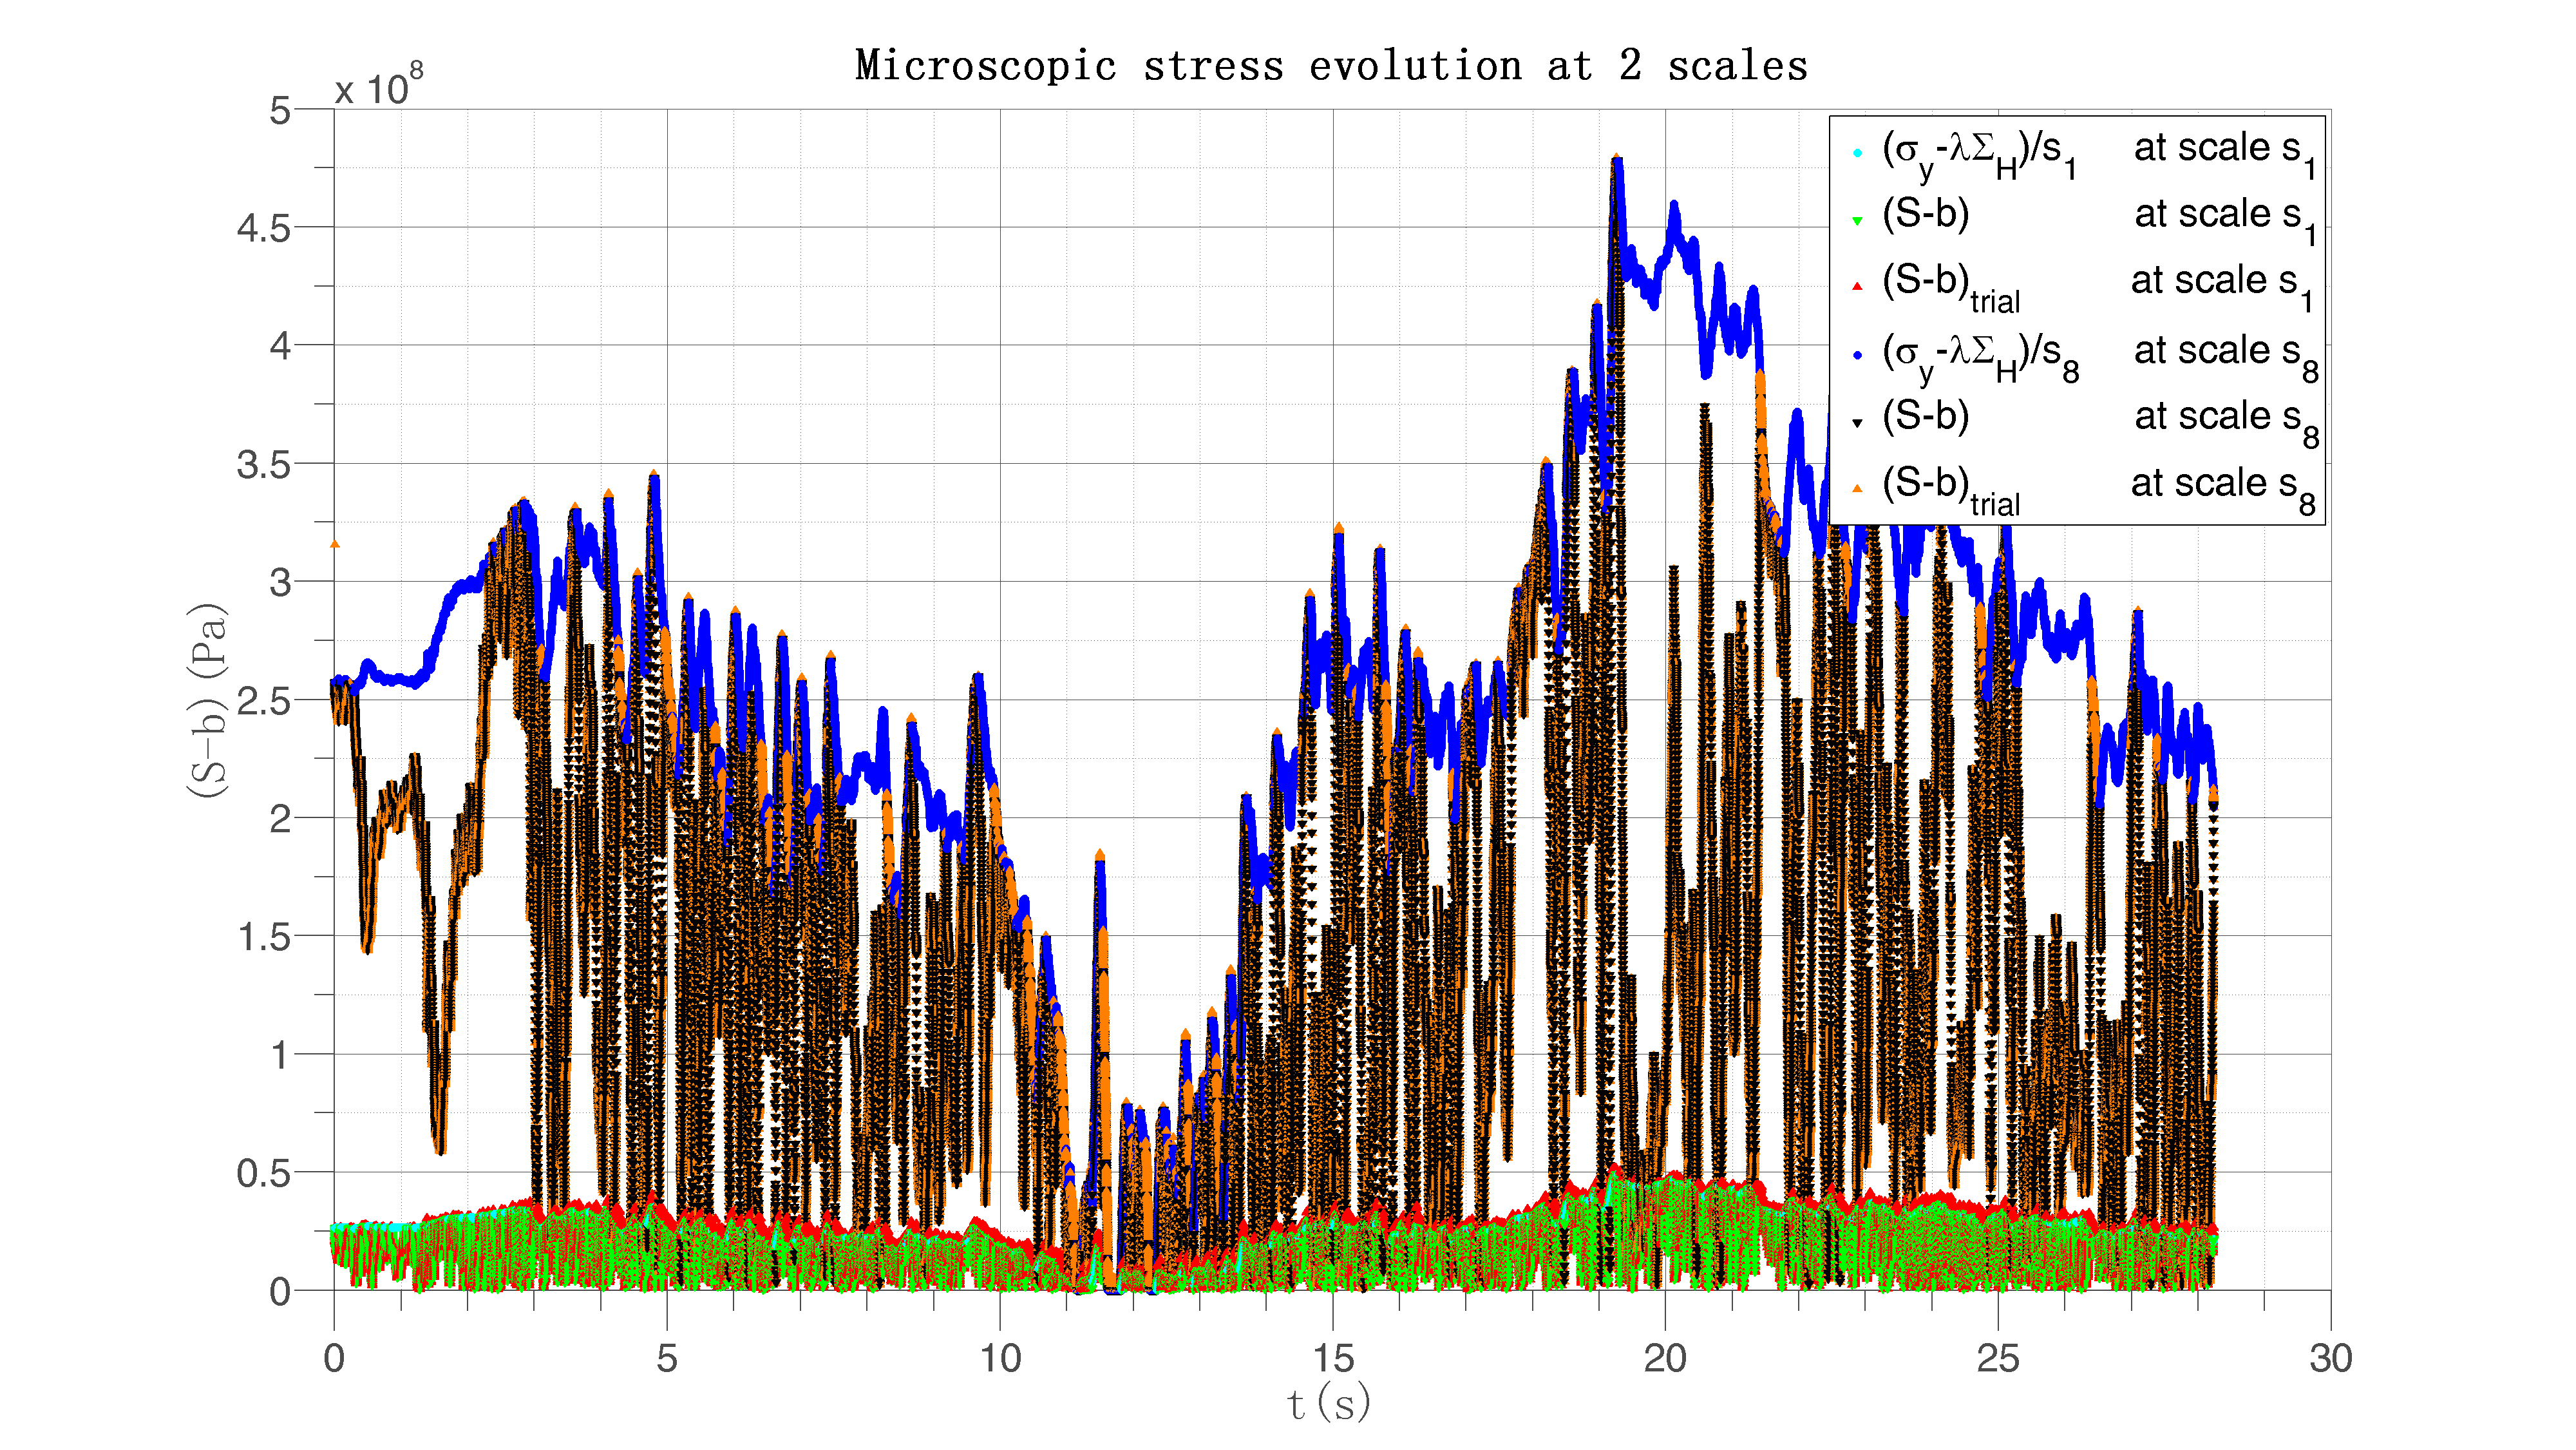
\includegraphics[width=\textwidth]{figures//trialreal3d.png} 
	\caption{$\left\| \uline{\uline{S}}-\uline{\uline{b}}\right\|_{trial}$ and $\left\| \uline{\uline{S}}-\uline{\uline{b}}\right\|$ evolution with time under different weakening scales in PSA load history}
	\label{trialreal3d2}
\end{figure} 
\end{frame}	
\begin{frame}
	\frametitle{Multi-dimensional application}
\begin{figure}[!h]
	\centering
	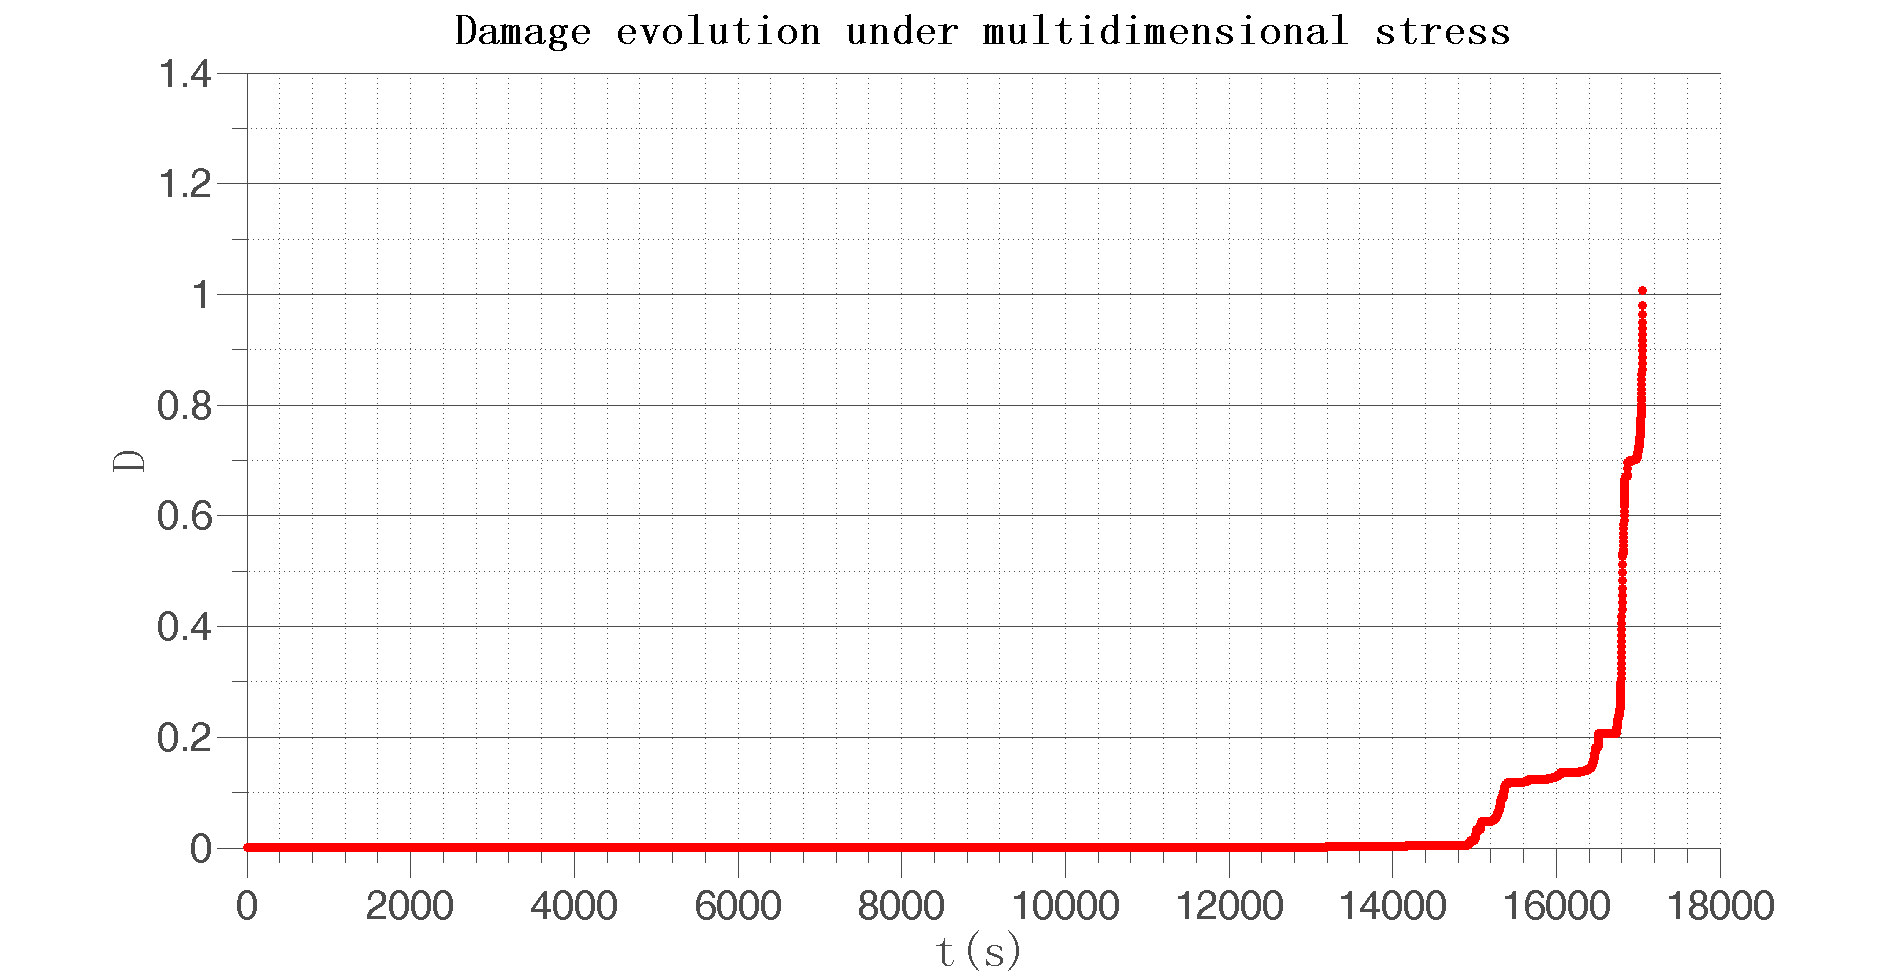
\includegraphics[width=\textwidth]{figures//damage3d2.png} 
	\caption{Damage evolution under multidimensional stress}
	\label{dam3d}
\end{figure}
\end{frame}	


\begin{frame}
	\frametitle{Results and discussion}	
		\begin{exampleblock}{ Results and discussion}
\begin{enumerate}
	\item We get rid of cycle counting method which for complex loading is hardly applicable.

	\vspace{6pt}
	\item The small step-by-step strategy does not ignore small fluctuations in load history and the big stress effect is magnified which reflects the real situation.
		
	\vspace{6pt}
	\item   The energy based fatigue approach takes into account impurities and hardness in the material and is applicable to any type of micro plasticity law and multiaxial load geometry.
	

	
\end{enumerate}
\end{exampleblock}
\end{frame}	


\begin{frame}
	\frametitle{}	
	\begin{exampleblock}{}
		{
			\Huge $$Thanks \, for \, your \, attention!$$
		}	  
	\end{exampleblock}
\end{frame}			
\end{document}

